\section{Messaufbau Resultate}
In diesem Kapitel werden die Messresultate des Laboraufbaus analysiert und mit den Simulationen und den Normen verglichen. Hierbei wurden die Daten der Messungen als .csv Datei gespeichert um mit Matlab die Signale schön darstellen zu können und das FFT berechnen zu können. 

\subsection{Messungen Widerstand}
Für die Messungen mit dem Widerstand, werden bei der Phasenanschnittsteuerung die Winkel 60\textdegree \hspace{0.02cm} und 90\textdegree \hspace{0.02cm} mit den Simulationen verglichen. Für die Schwingungspaketsteuerung wurde ein Duty cycle von 0.5 und 0.8 verglichen. Desweiteren werden noch der normale und der Langsame Sanft-Anlasser analysiert.
\subsubsection{Phasenanschnitt 60\textdegree}

\begin{figure}[ht!]
	\centering
	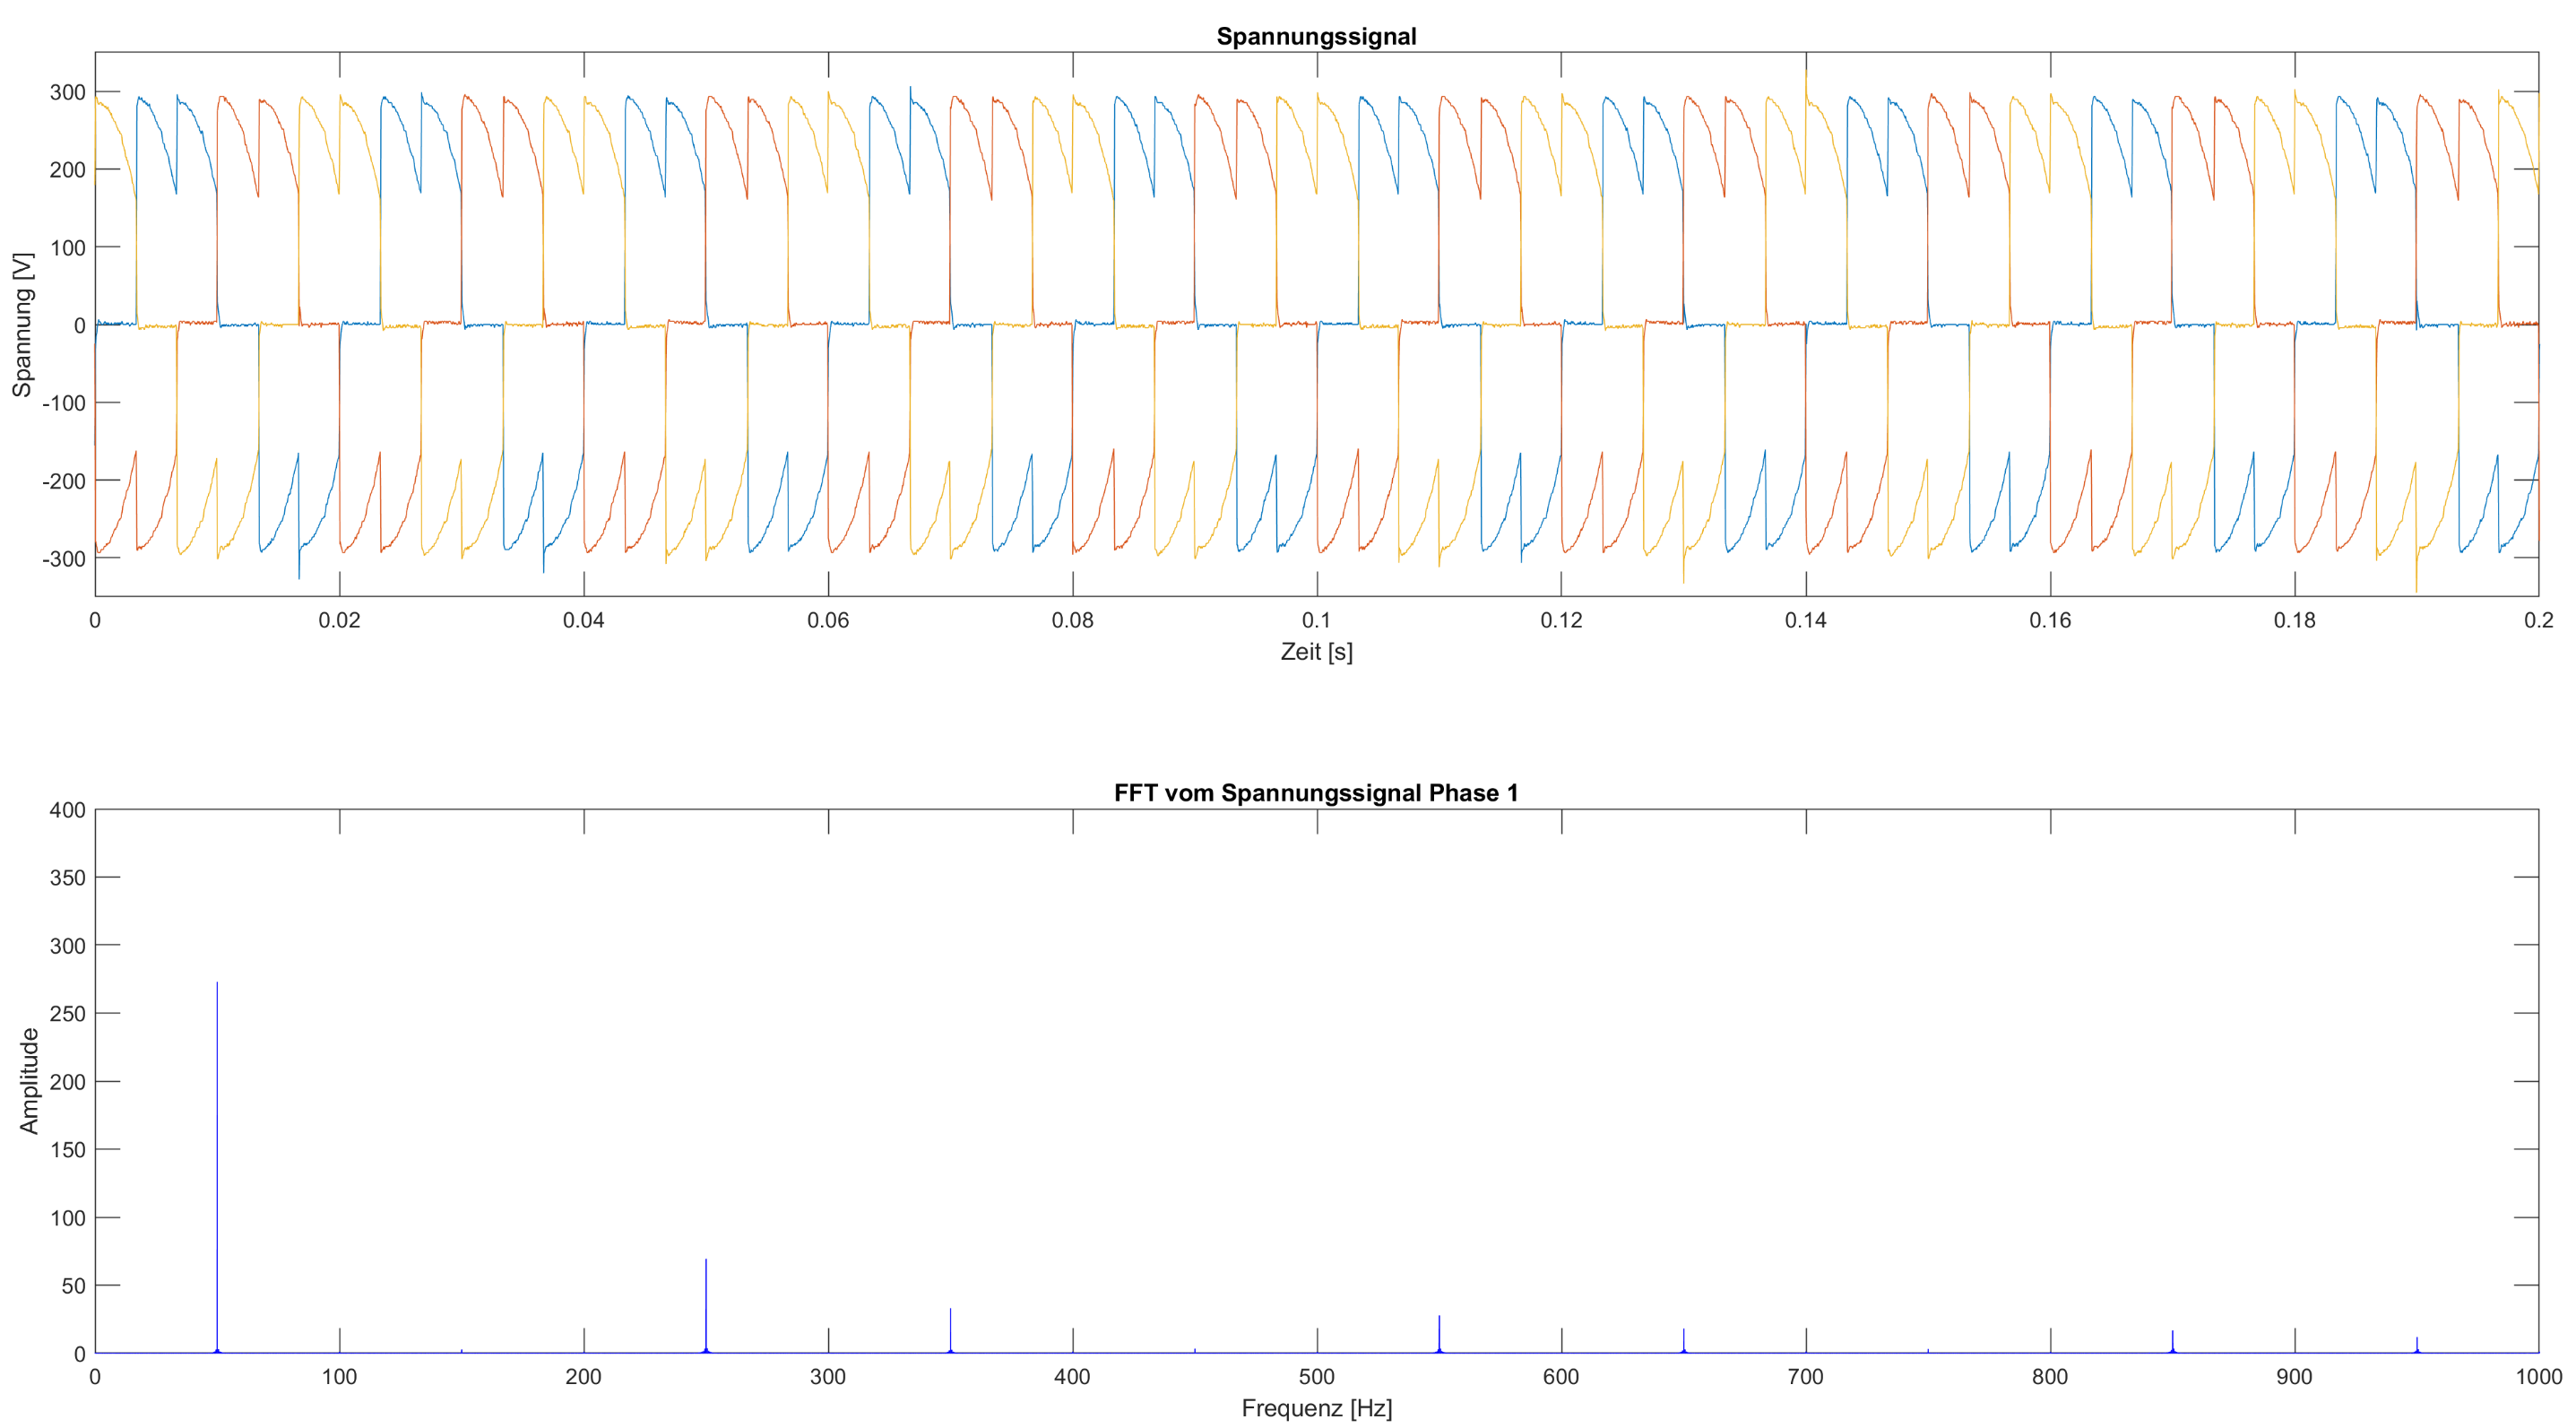
\includegraphics[width=\textwidth]{Messung_Widerstand_Phas_60grad.png}	
	\caption{Messung mit Phasenanschnitt 60\textdegree}\label{fig:Mess_Phas_60}
\end{figure}
\newpage
\subsubsection{Phasenanschnitt 90\textdegree}
\begin{figure}[ht!]
	\centering
	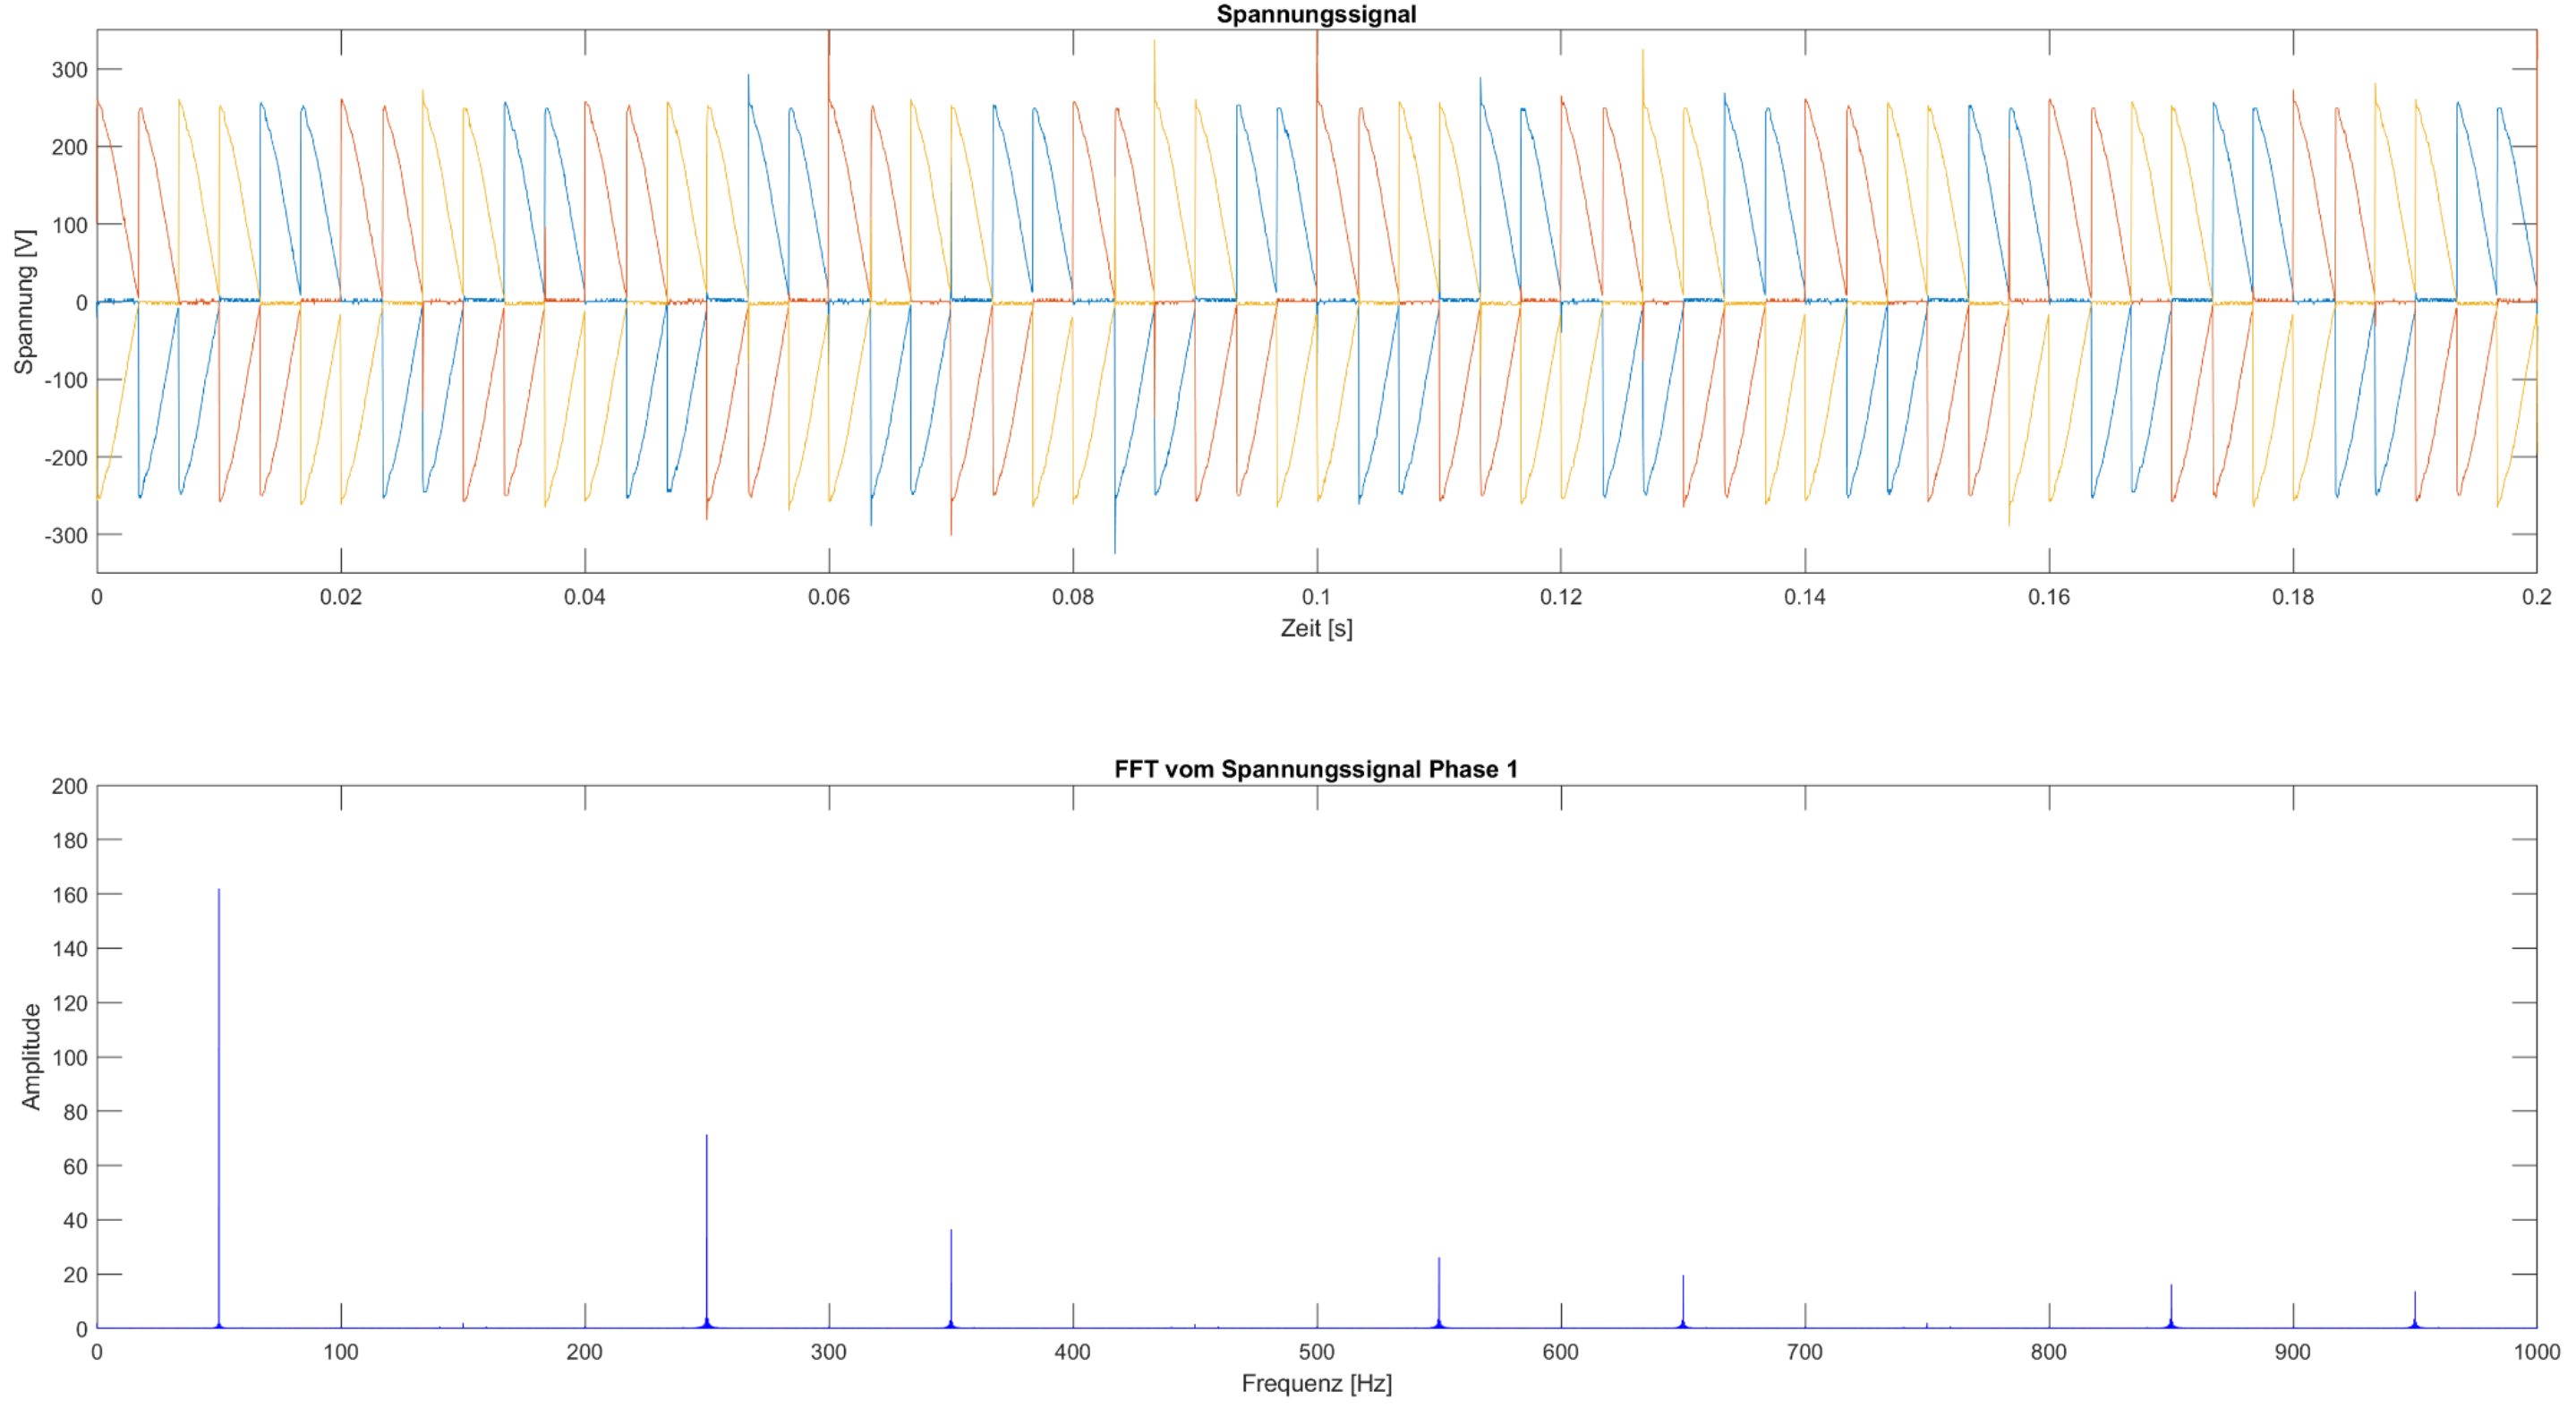
\includegraphics[width=\textwidth]{Messung_Widerstand_Phas_90grad.png}	
	\caption{Messung mit Phasenanschnitt 90\textdegree}\label{fig:Mess_Phas_90}
\end{figure}

\newpage
\subsubsection{Schwingungspaket 50\%}
\begin{figure}[ht!]
	\centering
	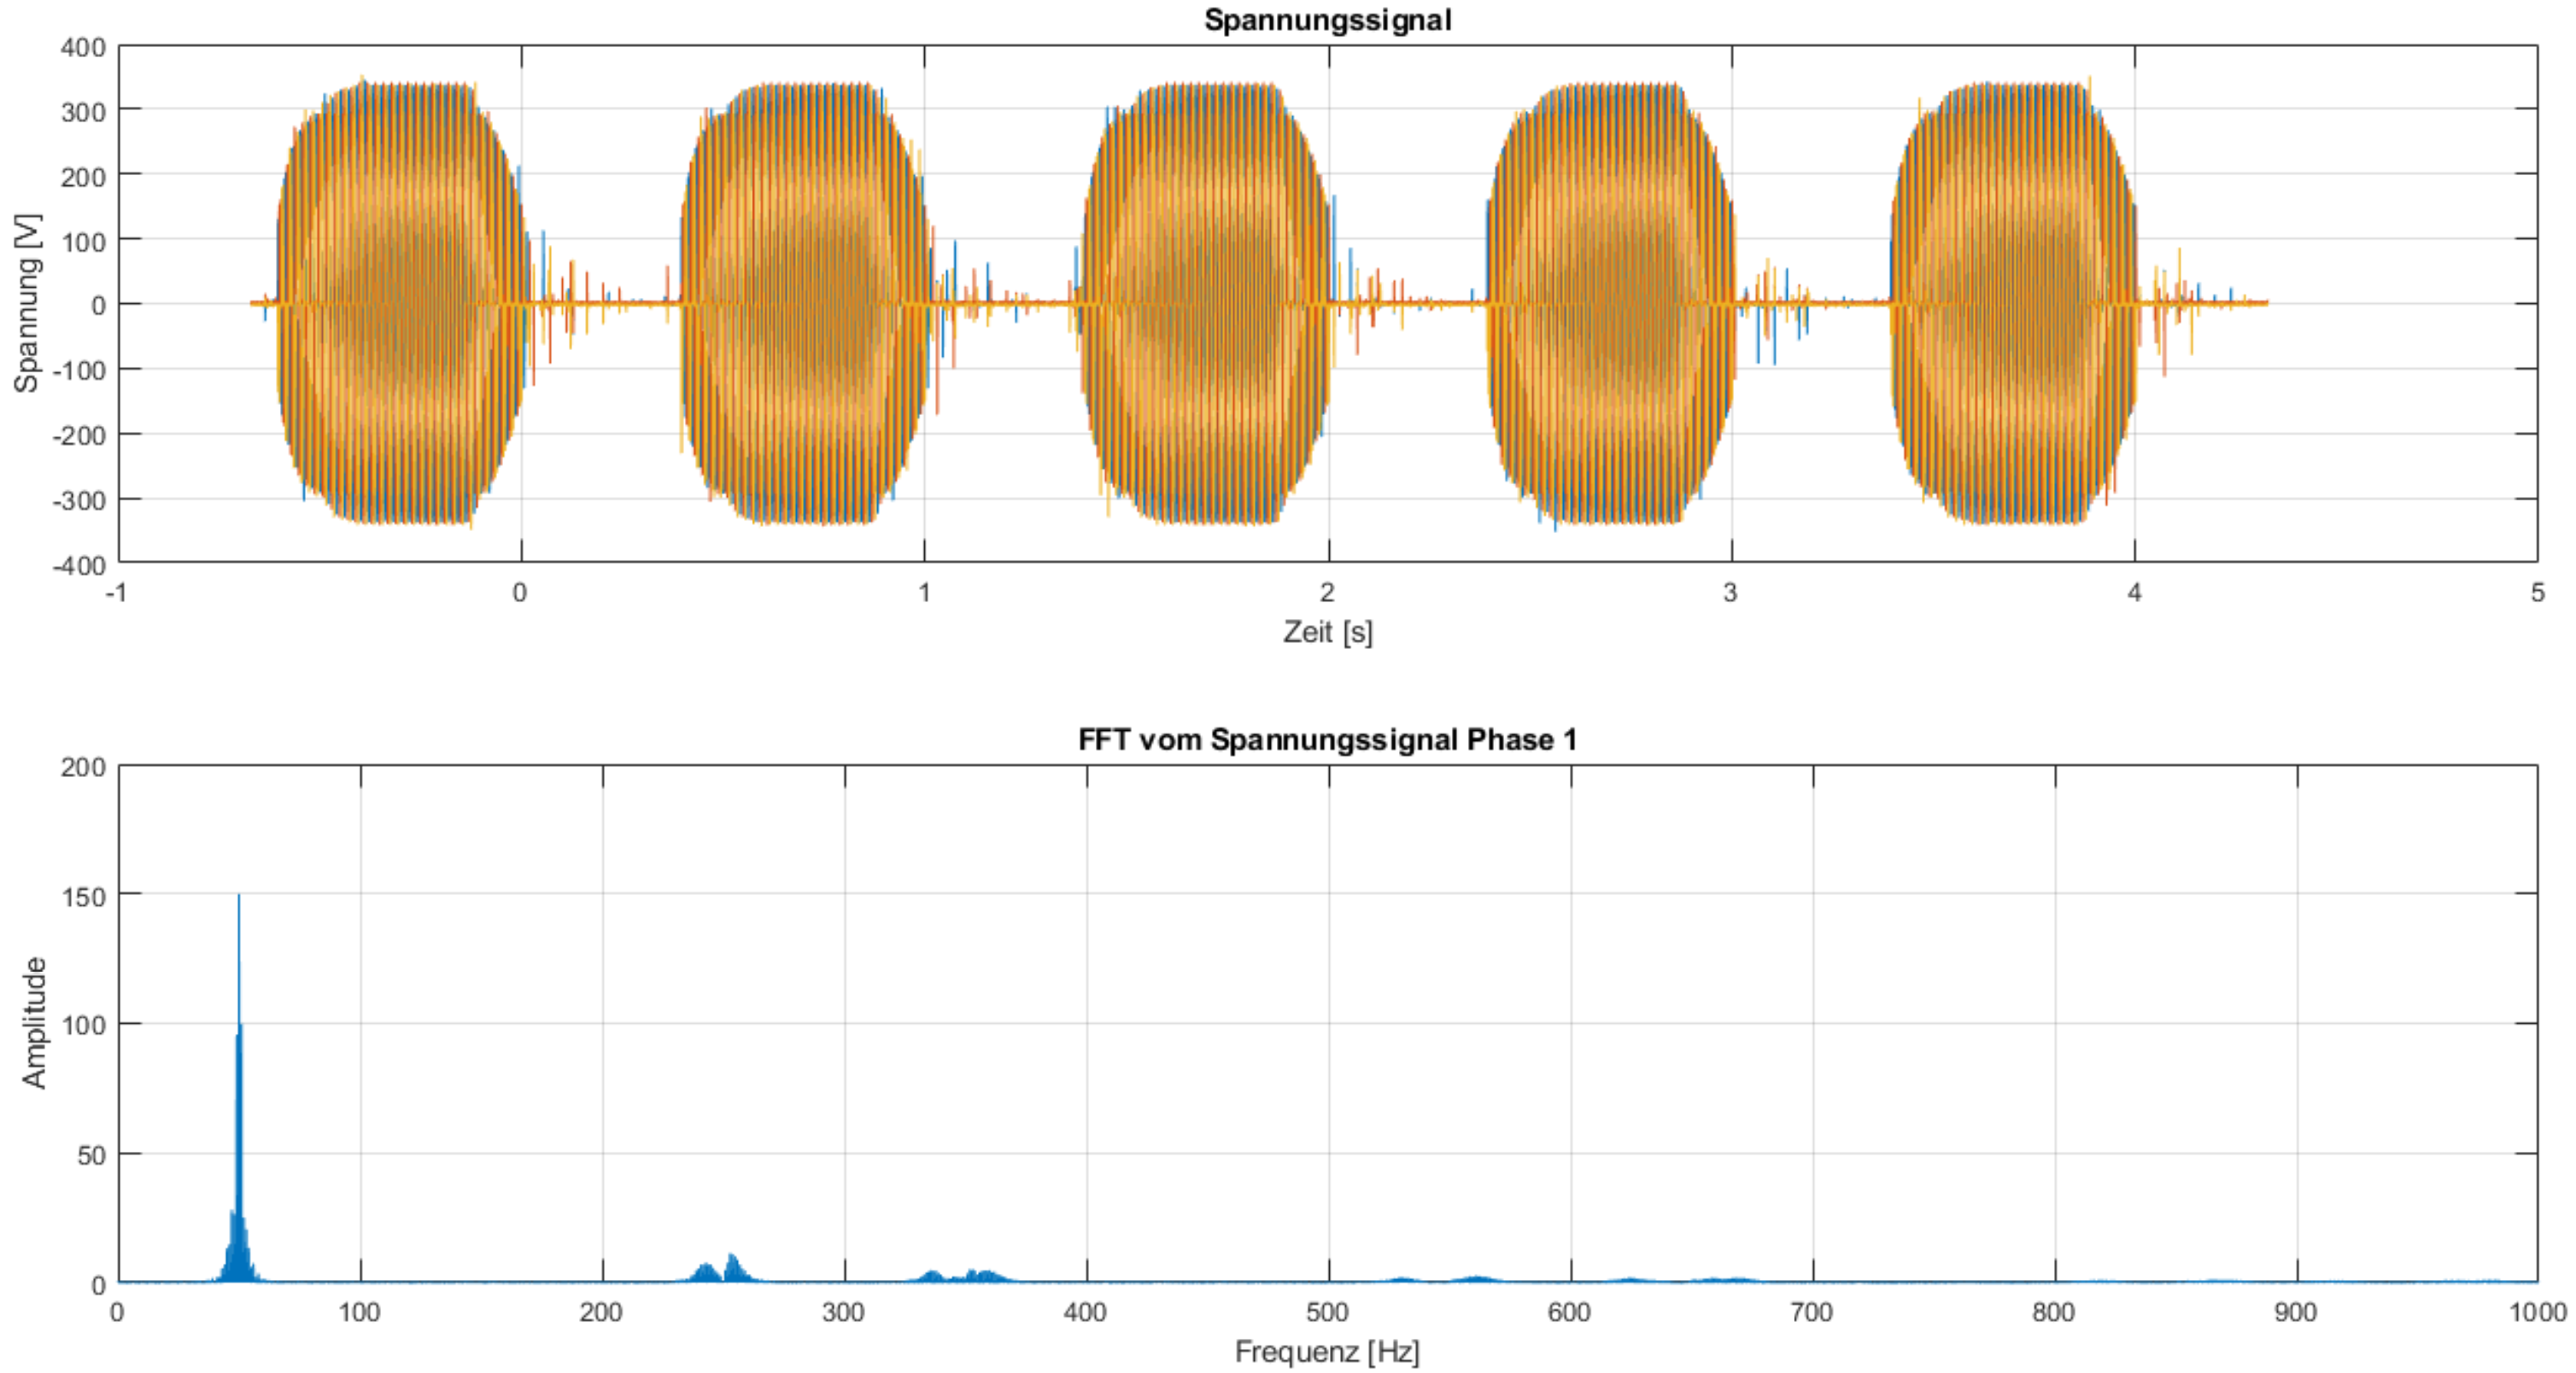
\includegraphics[width=\textwidth]{Messung_Widerstand_Schwing_0_5.png}	
	\caption{Messung mit Phasenanschnitt 90\textdegree}\label{fig:Mess_Schwing_50}
\end{figure}

\newpage
\subsubsection{Schwingungspaket 80\%}
\begin{figure}[ht!]
	\centering
	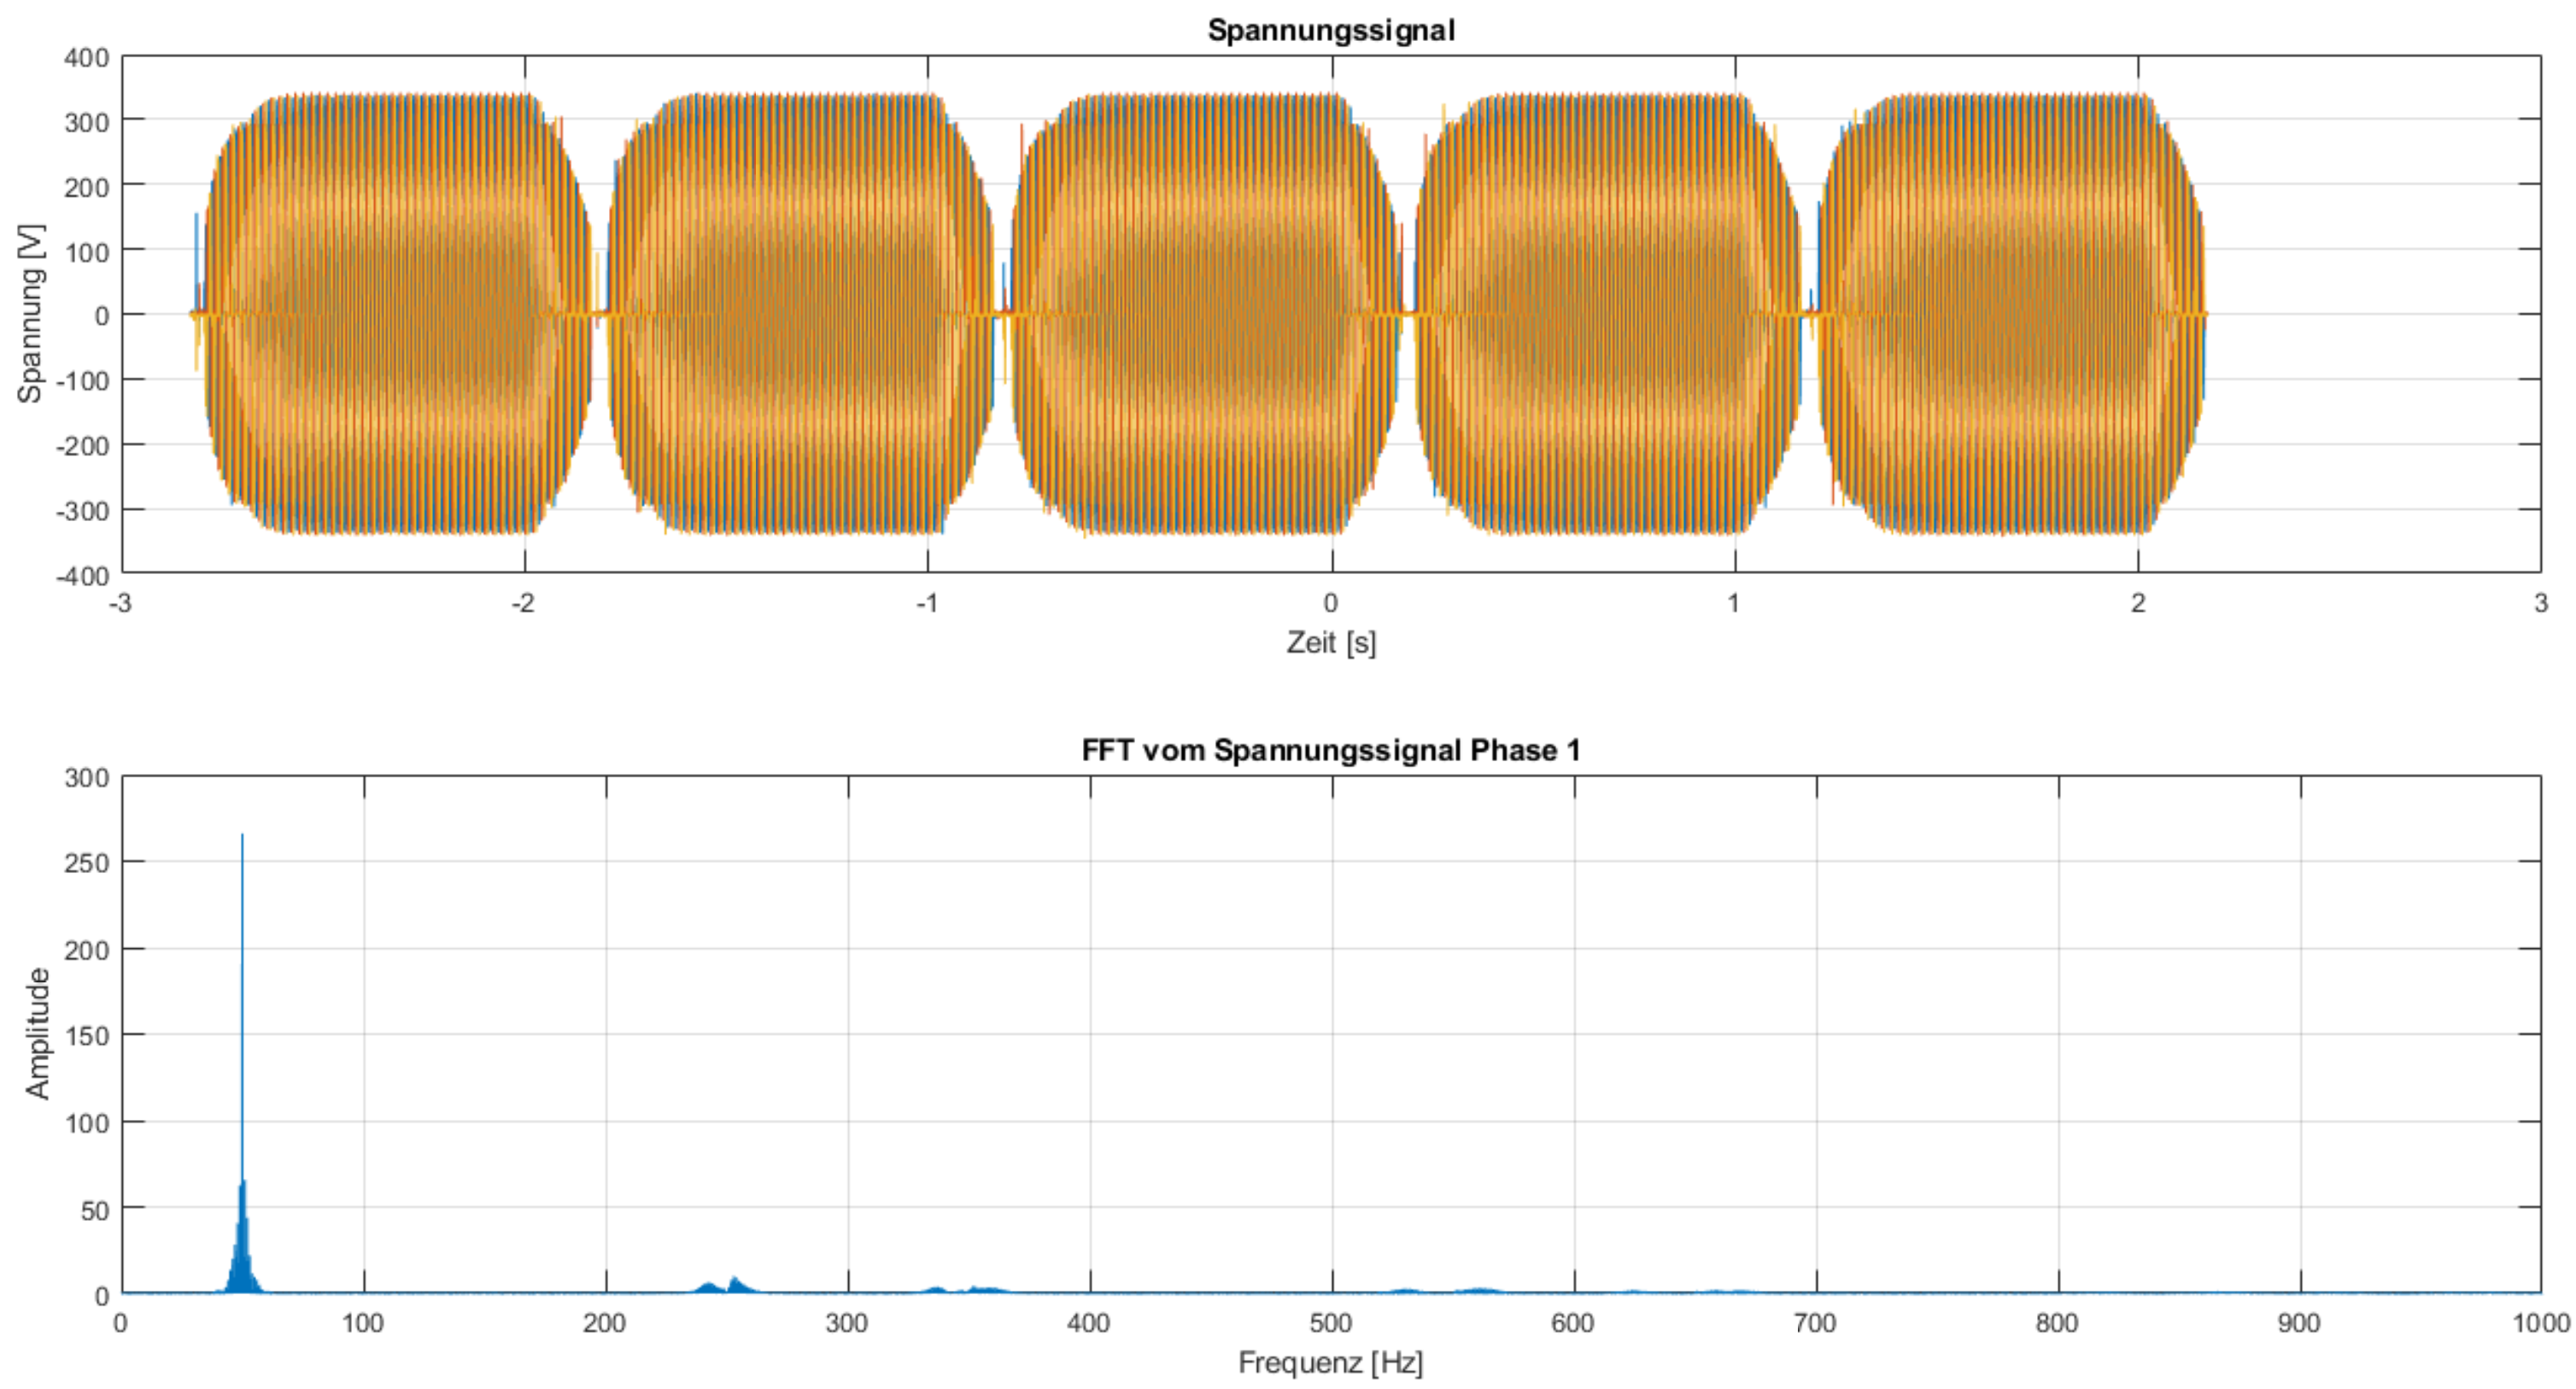
\includegraphics[width=\textwidth]{Messung_Widerstand_Schwing_0_8.png}	
	\caption{Messung mit Phasenanschnitt 90\textdegree}\label{fig:Mess_Schwing_80}
\end{figure}

\newpage
\subsubsection{Sanft-Anlasser}
\begin{figure}[ht!]
	\centering
	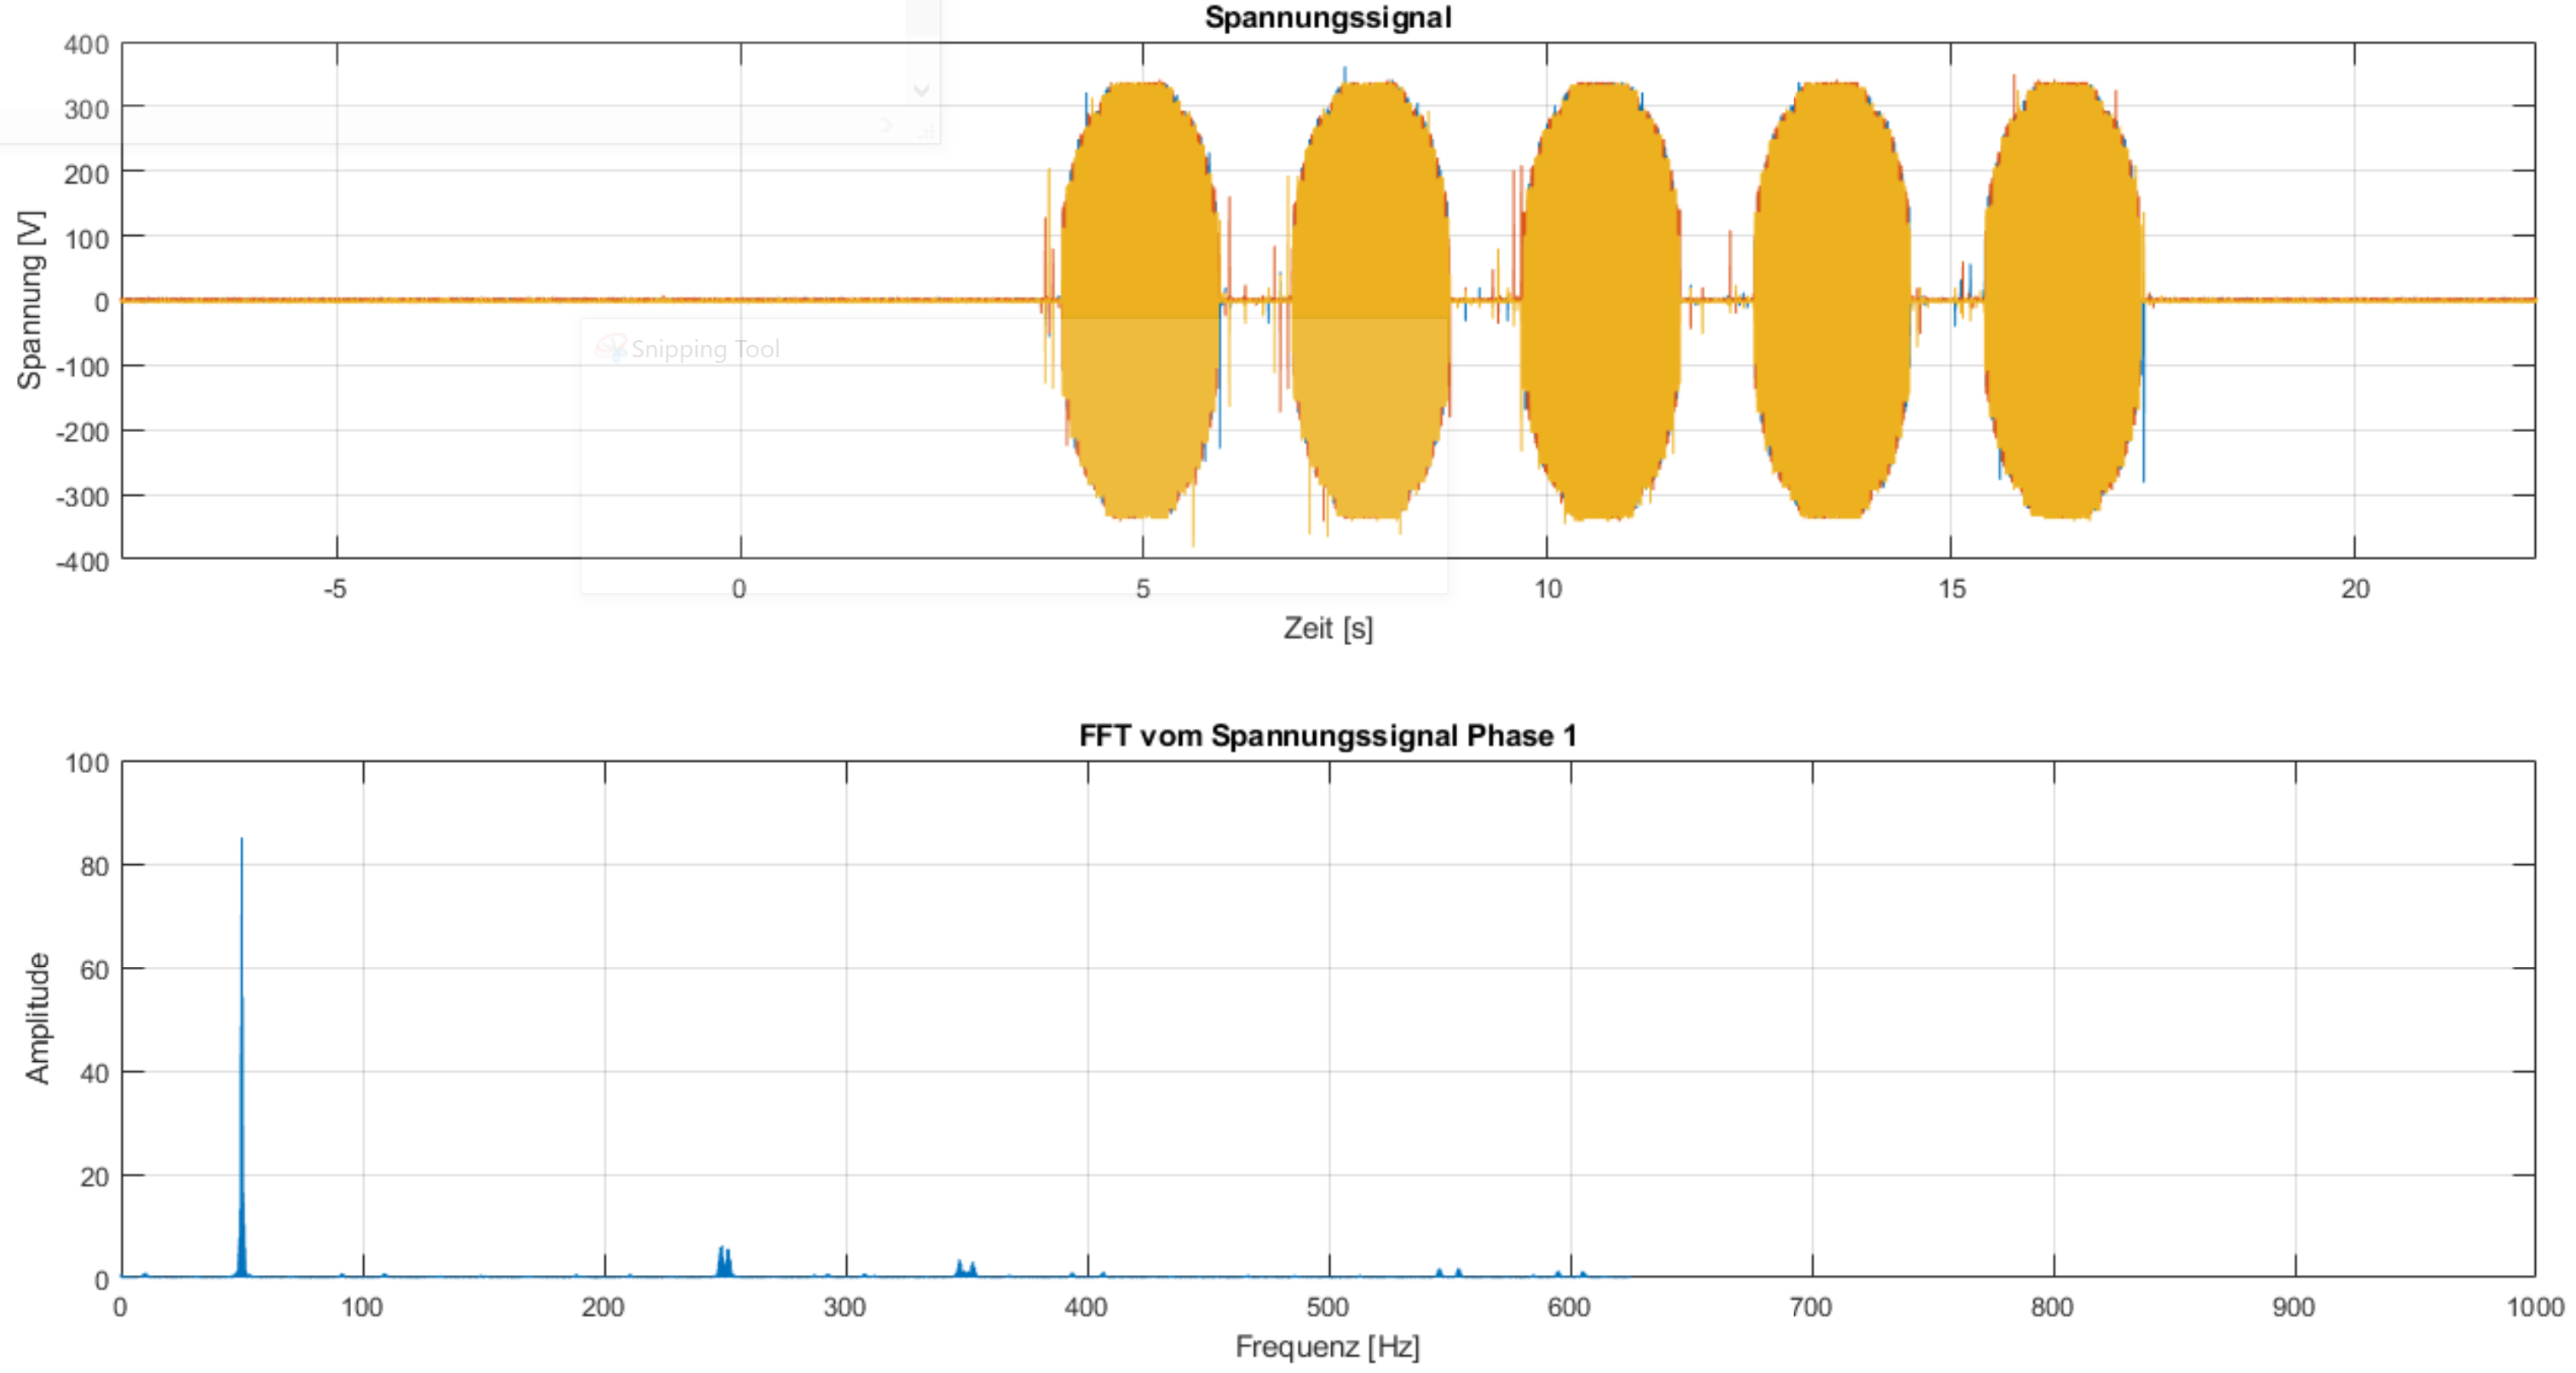
\includegraphics[width=\textwidth]{Messung_Widerstand_Sanft.png}	
	\caption{Messung mit Phasenanschnitt 90\textdegree}\label{fig:Mess_Sanft}
\end{figure}

\newpage
\subsubsection{Sanft-Anlasser Langsam}
\begin{figure}[ht!]
	\centering
	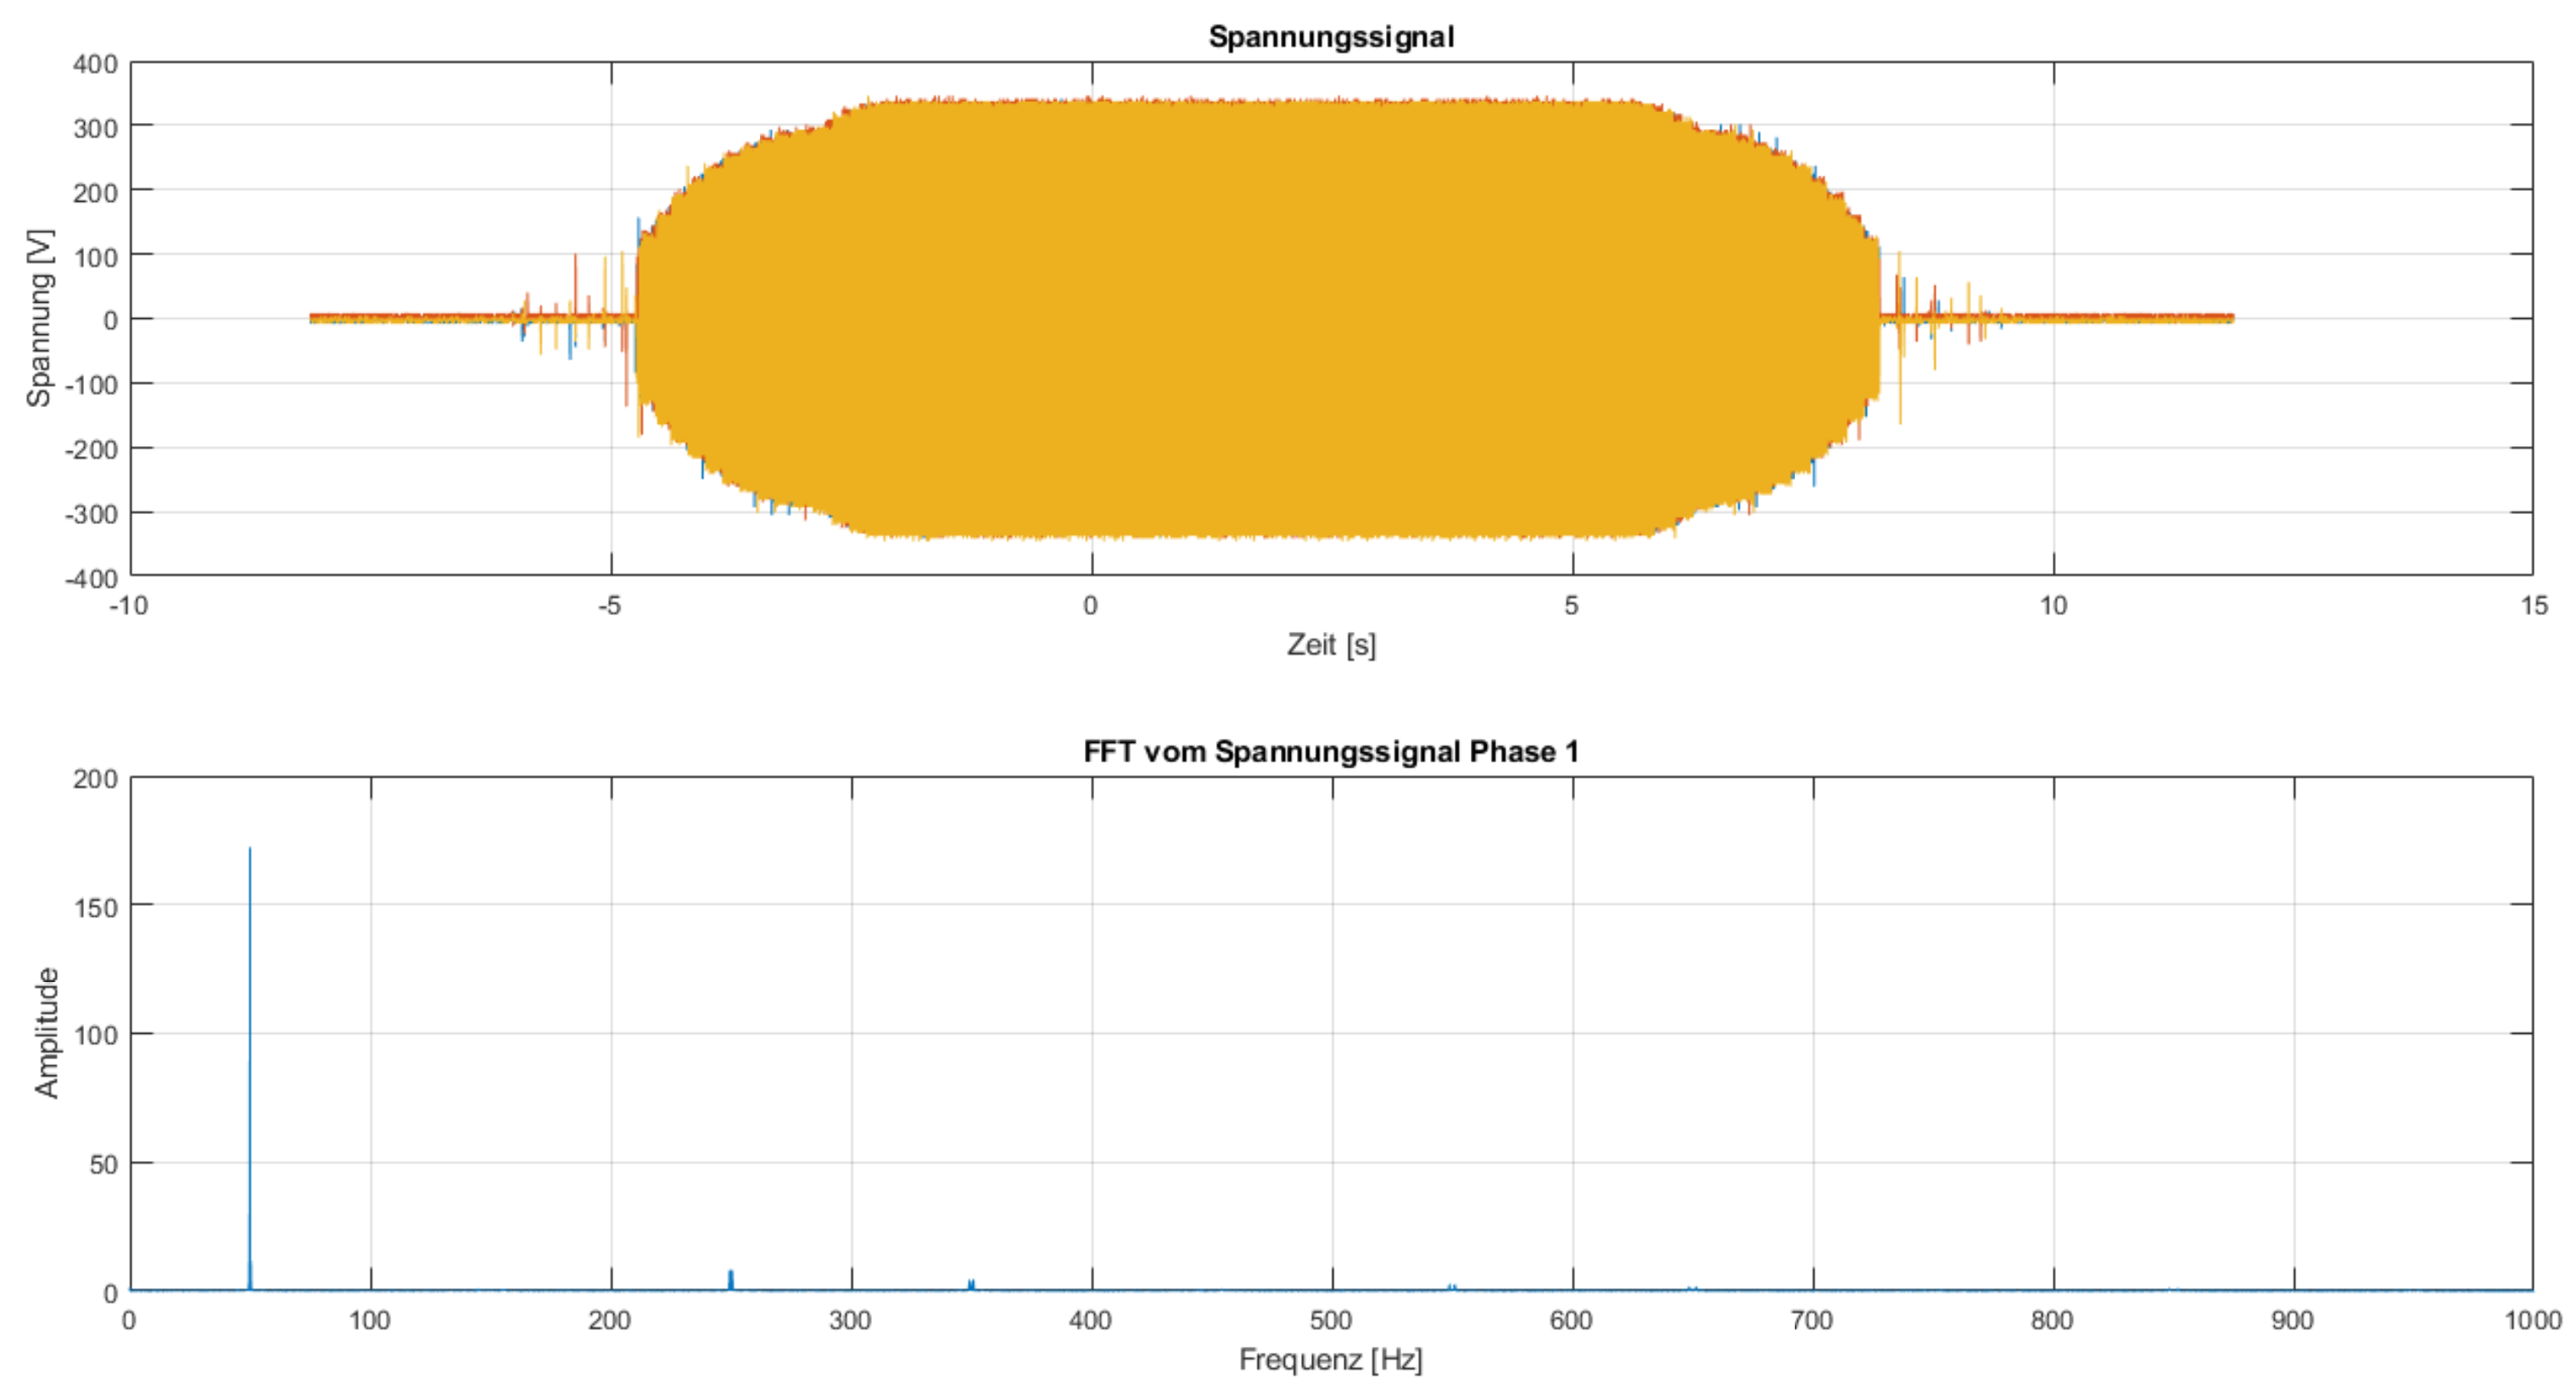
\includegraphics[width=\textwidth]{Messung_Widerstand_Sanft_langsam.png}	
	\caption{Messung mit Phasenanschnitt 90\textdegree}\label{fig:Mess_Sanft_langsam}
\end{figure}

\newpage
\subsection{Messungen ASM}

\subsubsection{Phasenanschnitt 60\textdegree}
\begin{figure}[ht!]
	\centering
	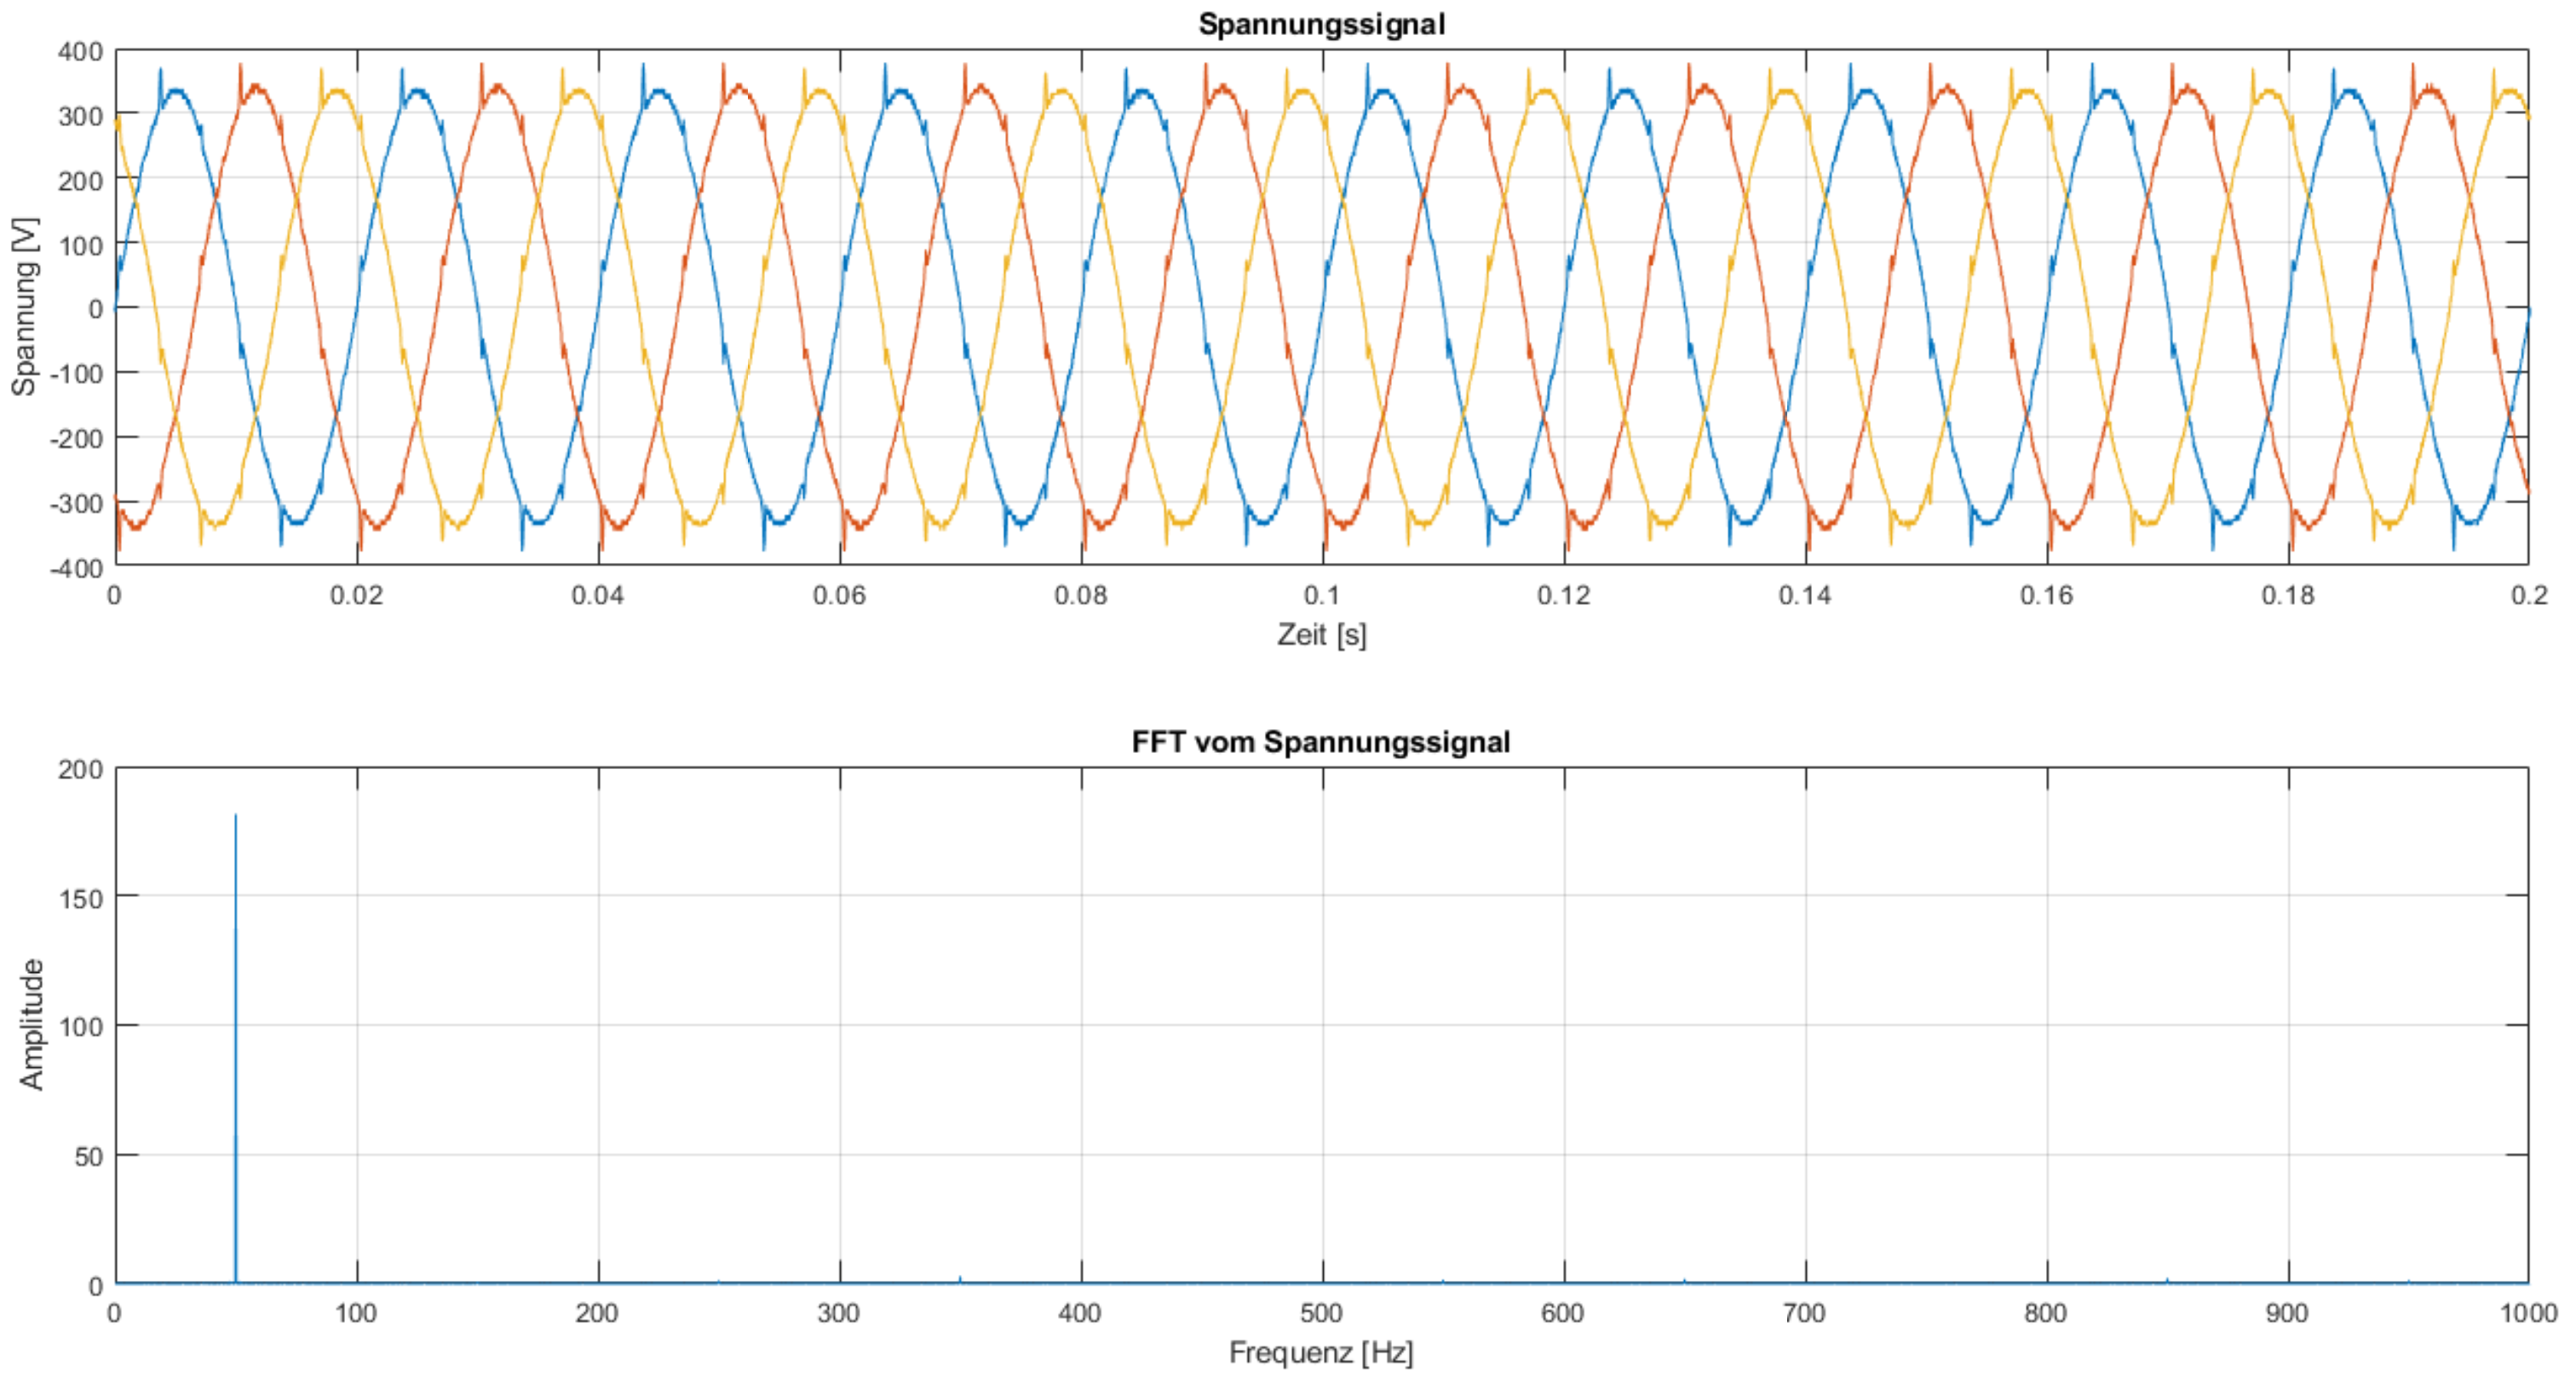
\includegraphics[width=\textwidth]{Messung_ASM_Phas_60grad.png}	
	\caption{Messung mit Phasenanschnitt 60\textdegree}\label{fig:Mess_ASM_Phas60}
\end{figure}

\newpage
\subsubsection{Phasenanschnitt 90\textdegree}
\begin{figure}[ht!]
	\centering
	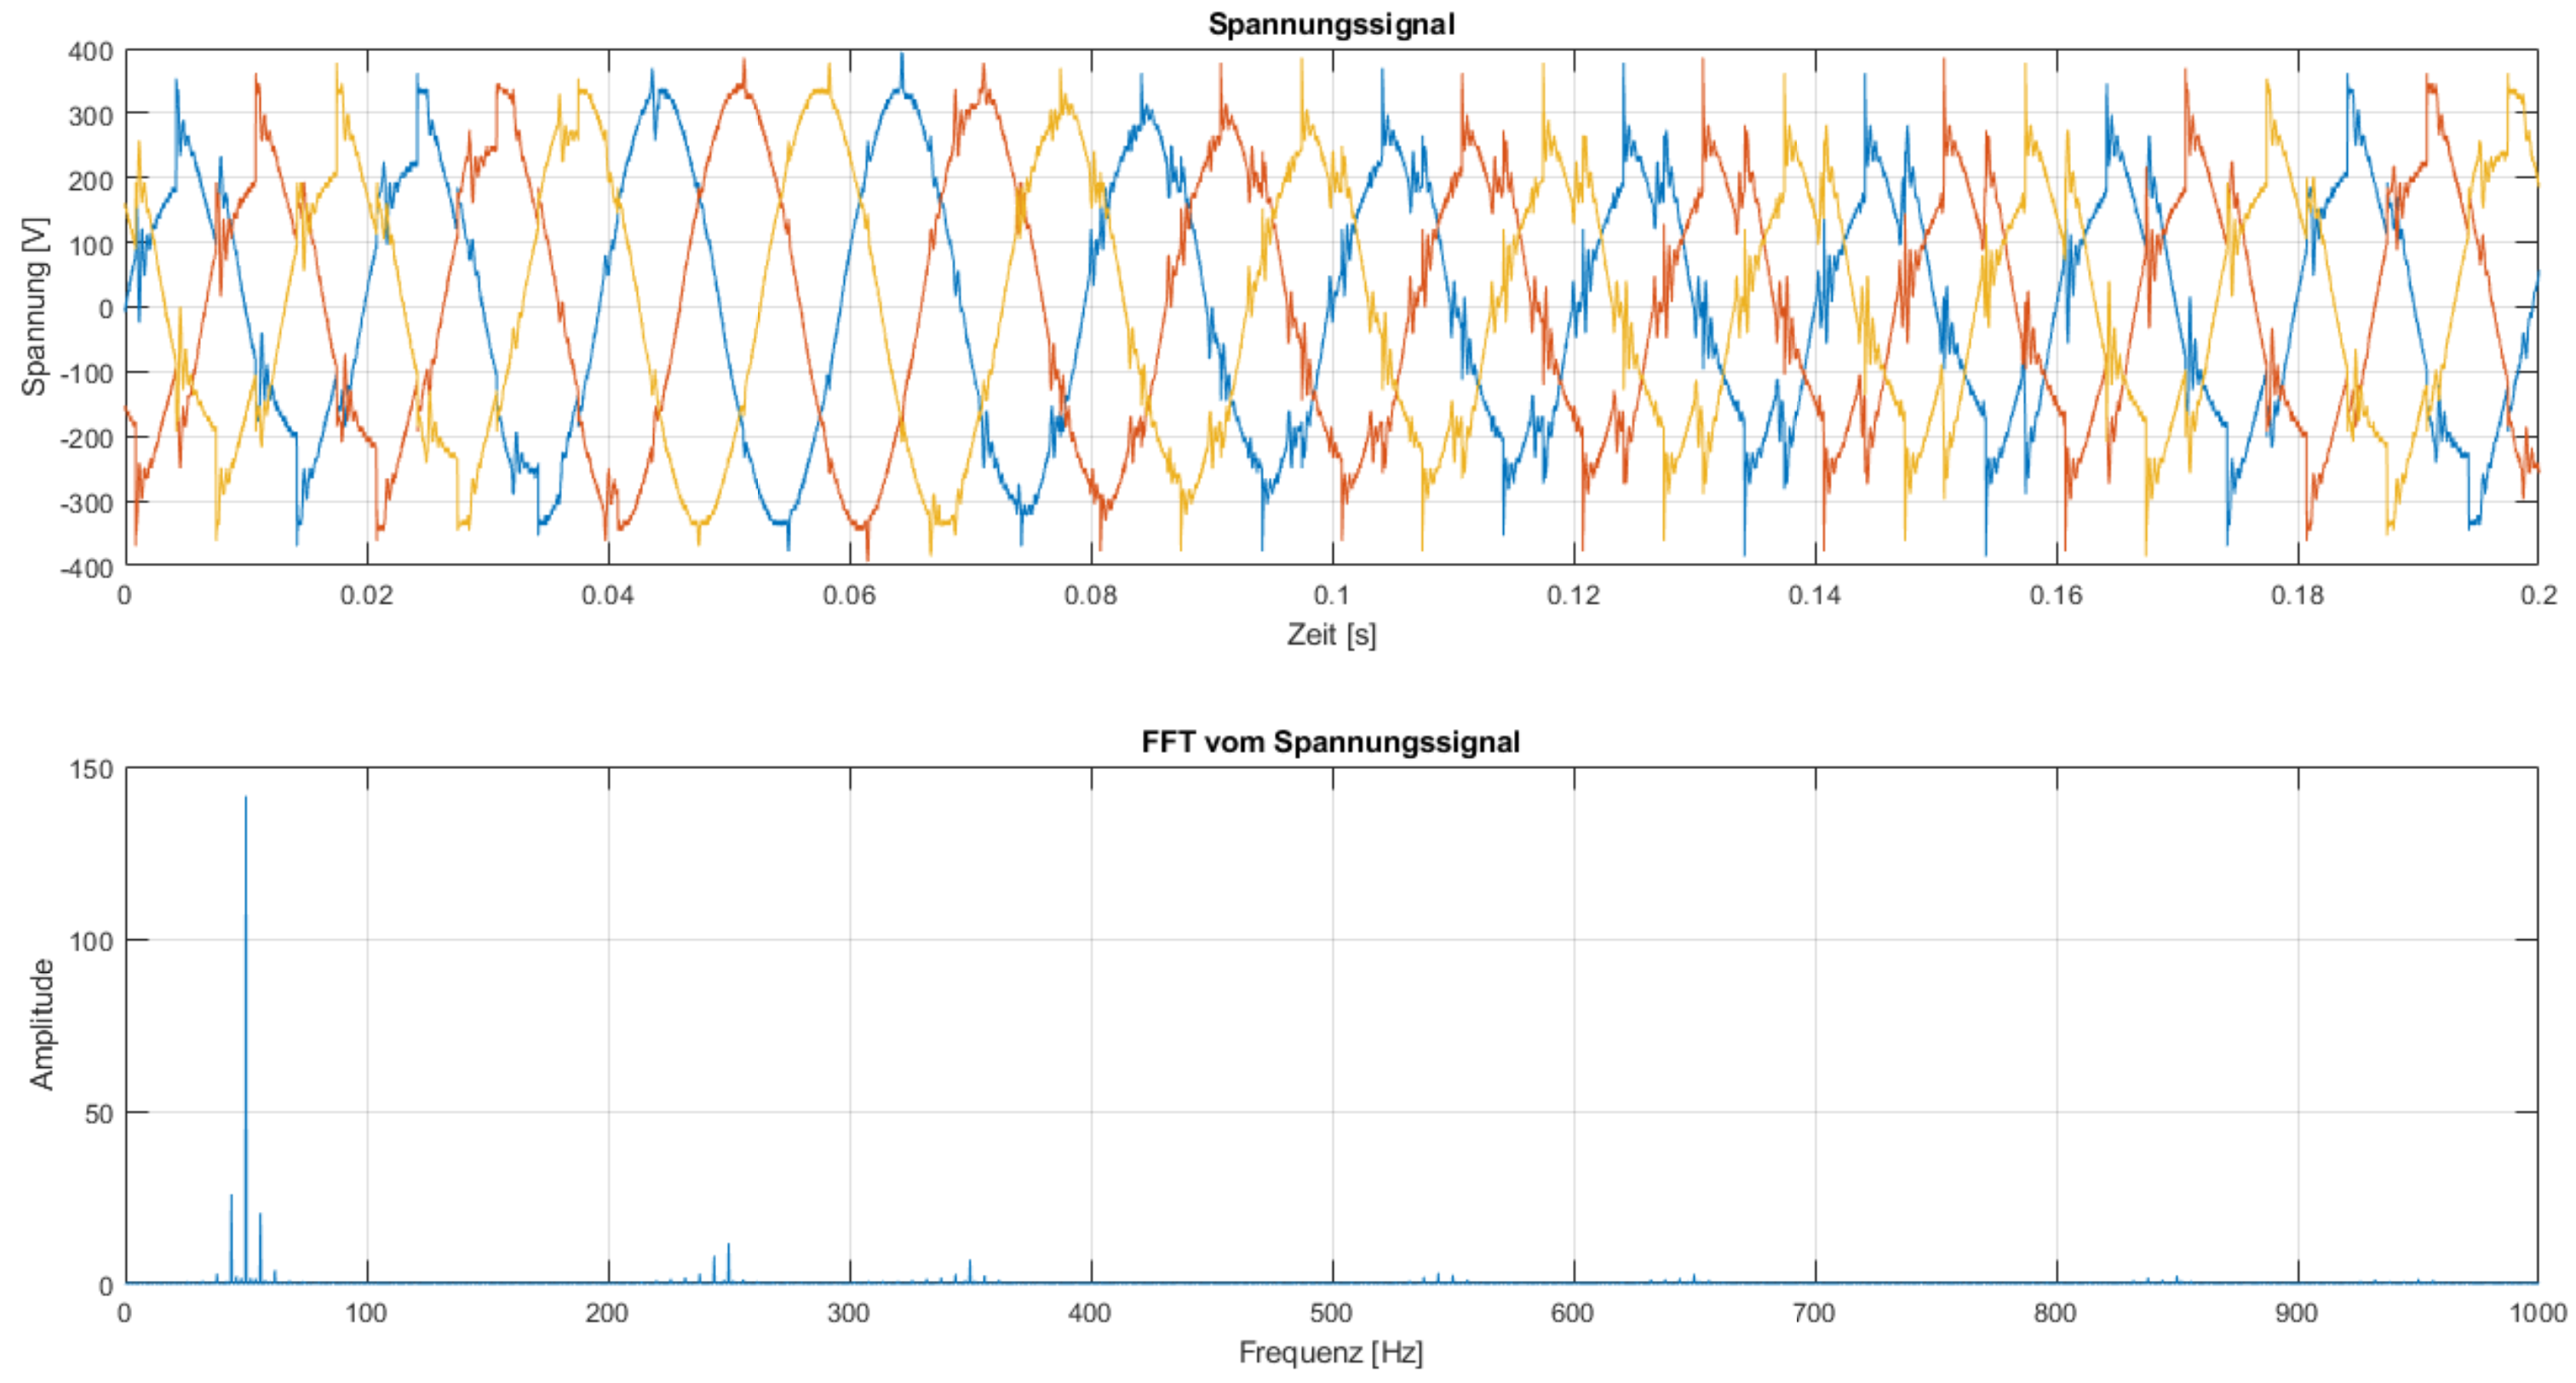
\includegraphics[width=\textwidth]{Messung_ASM_Phas_90grad.png}	
	\caption{Messung mit Phasenanschnitt 90\textdegree}\label{fig:Mess_ASM_Phas90}
\end{figure}

\newpage
\subsubsection{Schwingungspaket 50\%}
\begin{figure}[ht!]
	\centering
	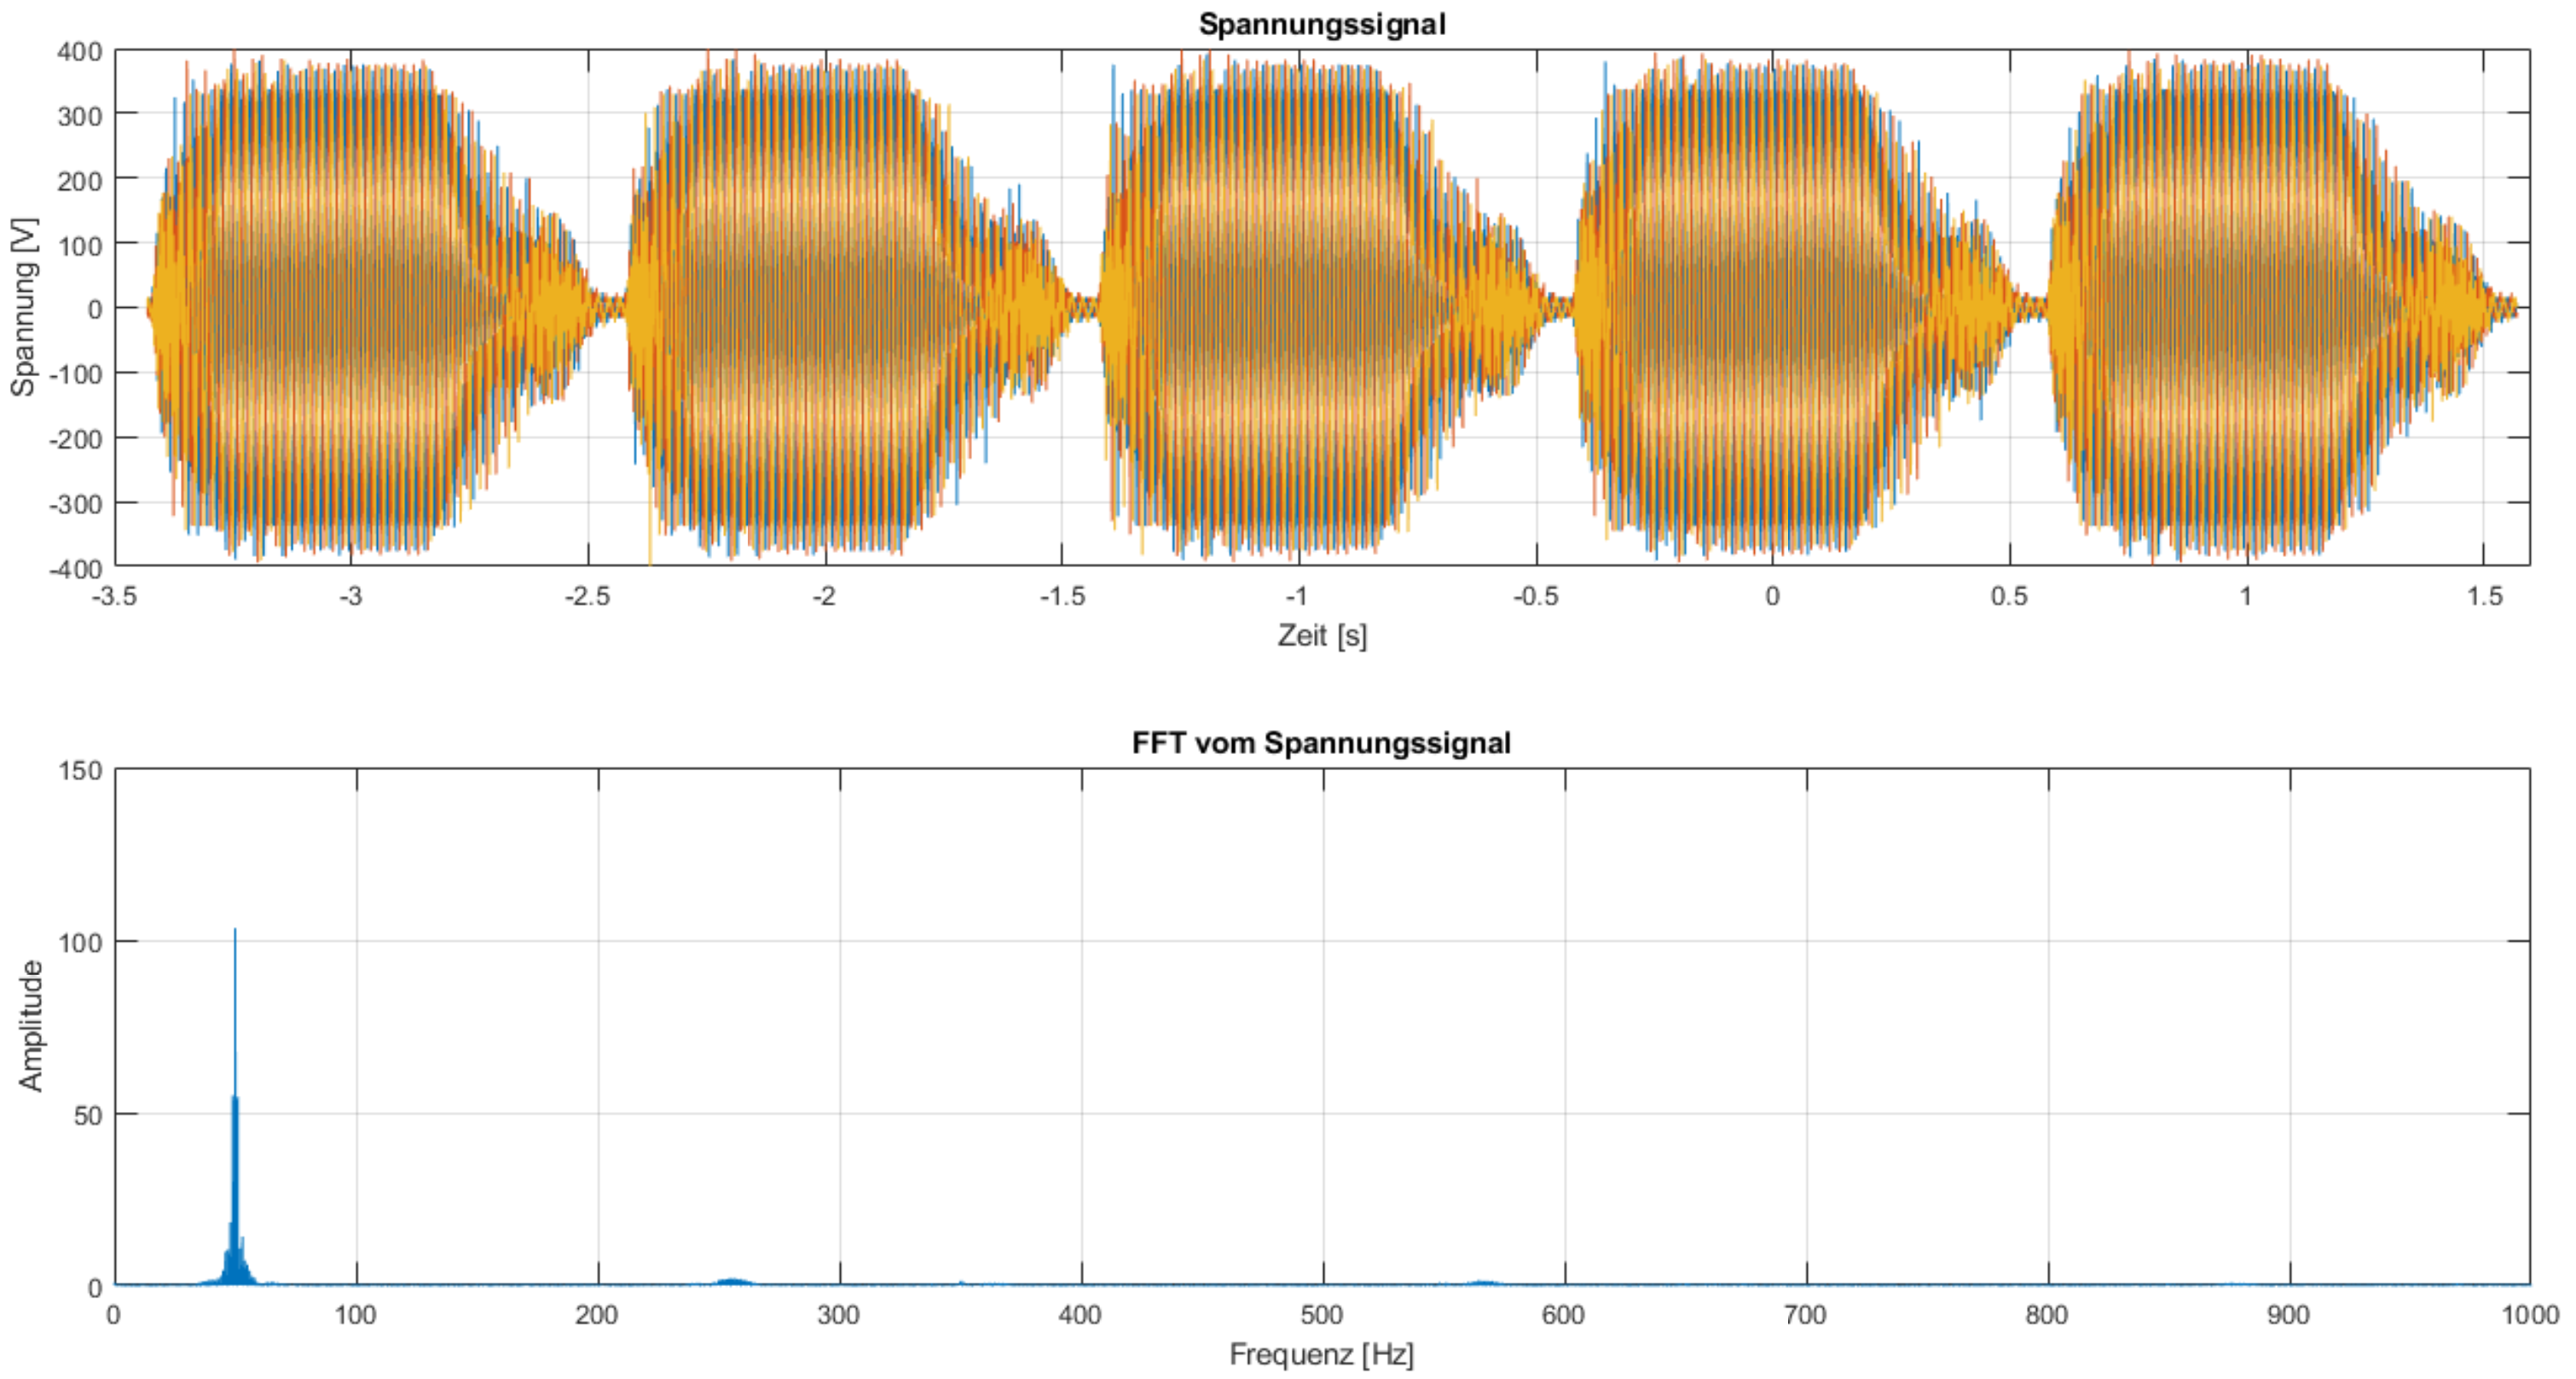
\includegraphics[width=\textwidth]{Messung_ASM_Schwing_0_5.png}	
	\caption{Messung mit Phasenanschnitt 90\textdegree}\label{fig:Mess_ASM_Schwing_0_5}
\end{figure}

\newpage
\subsubsection{Schwingungspaket 80\%}
\begin{figure}[ht!]
	\centering
	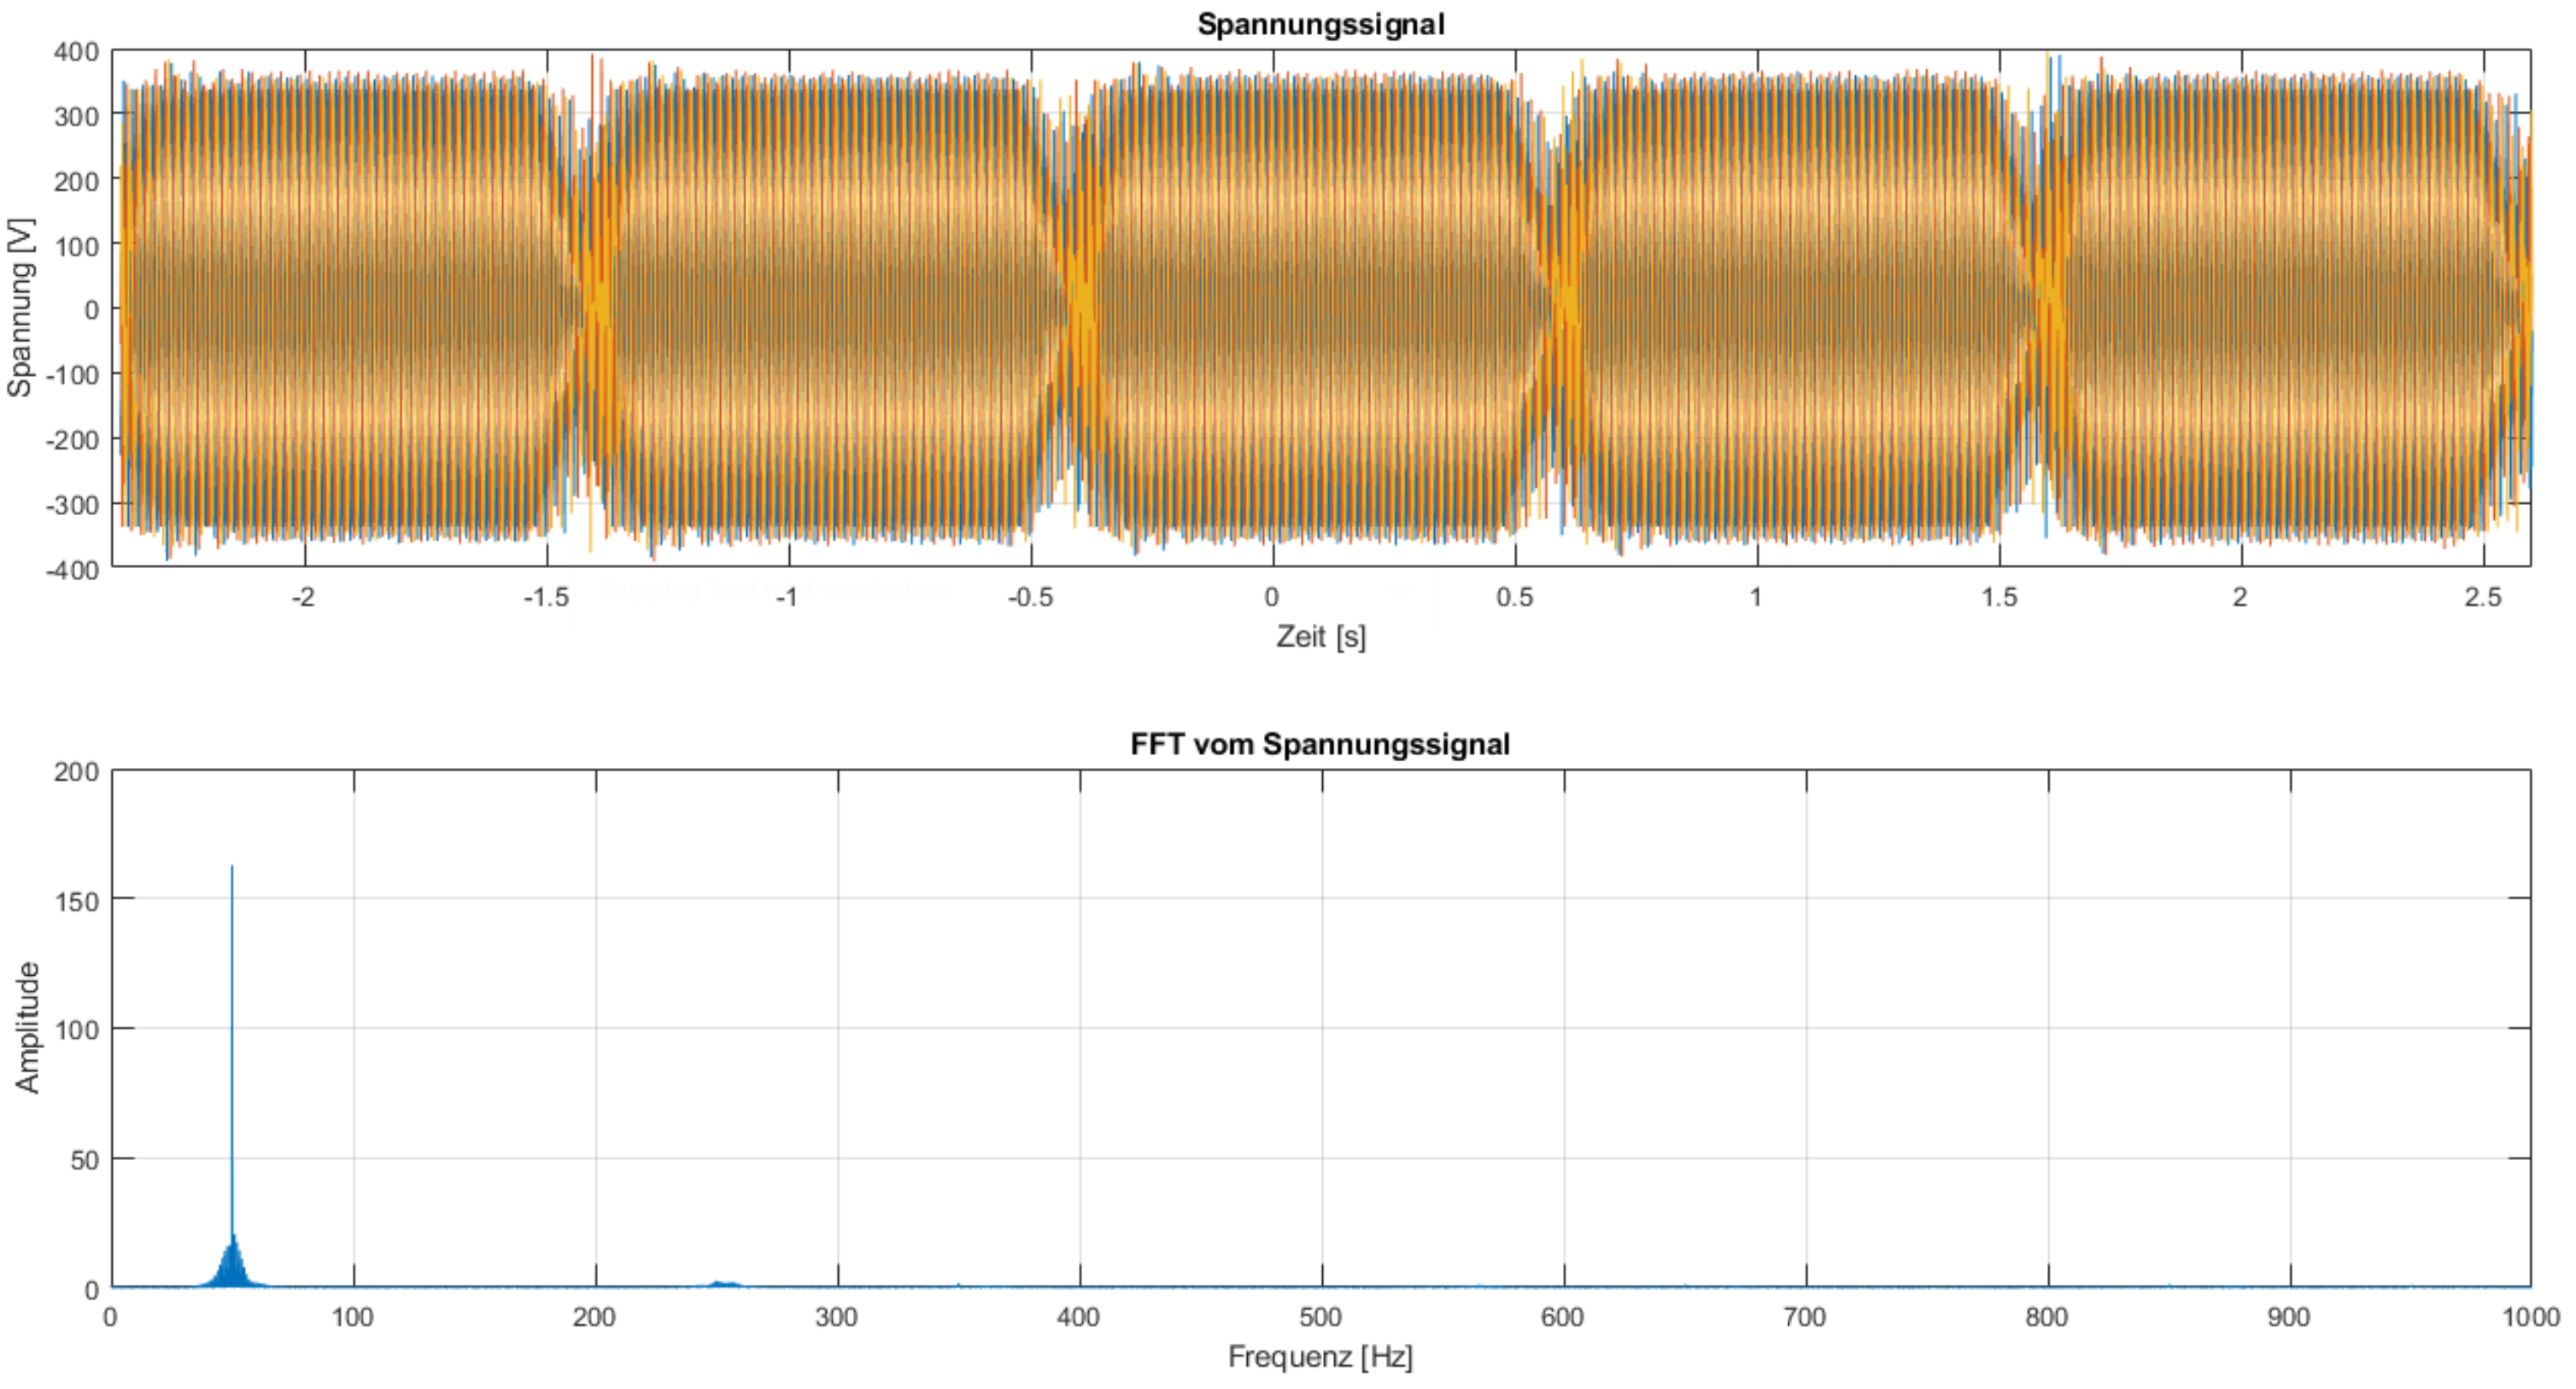
\includegraphics[width=\textwidth]{Messung_ASM_Schwing_0_8.png}	
	\caption{Messung mit Phasenanschnitt 90\textdegree}\label{fig:Mess_ASM_Schwing_0_8}
\end{figure}

\newpage
\subsubsection{Sanft-Anlasser Langsam}
\begin{figure}[ht!]
	\centering
	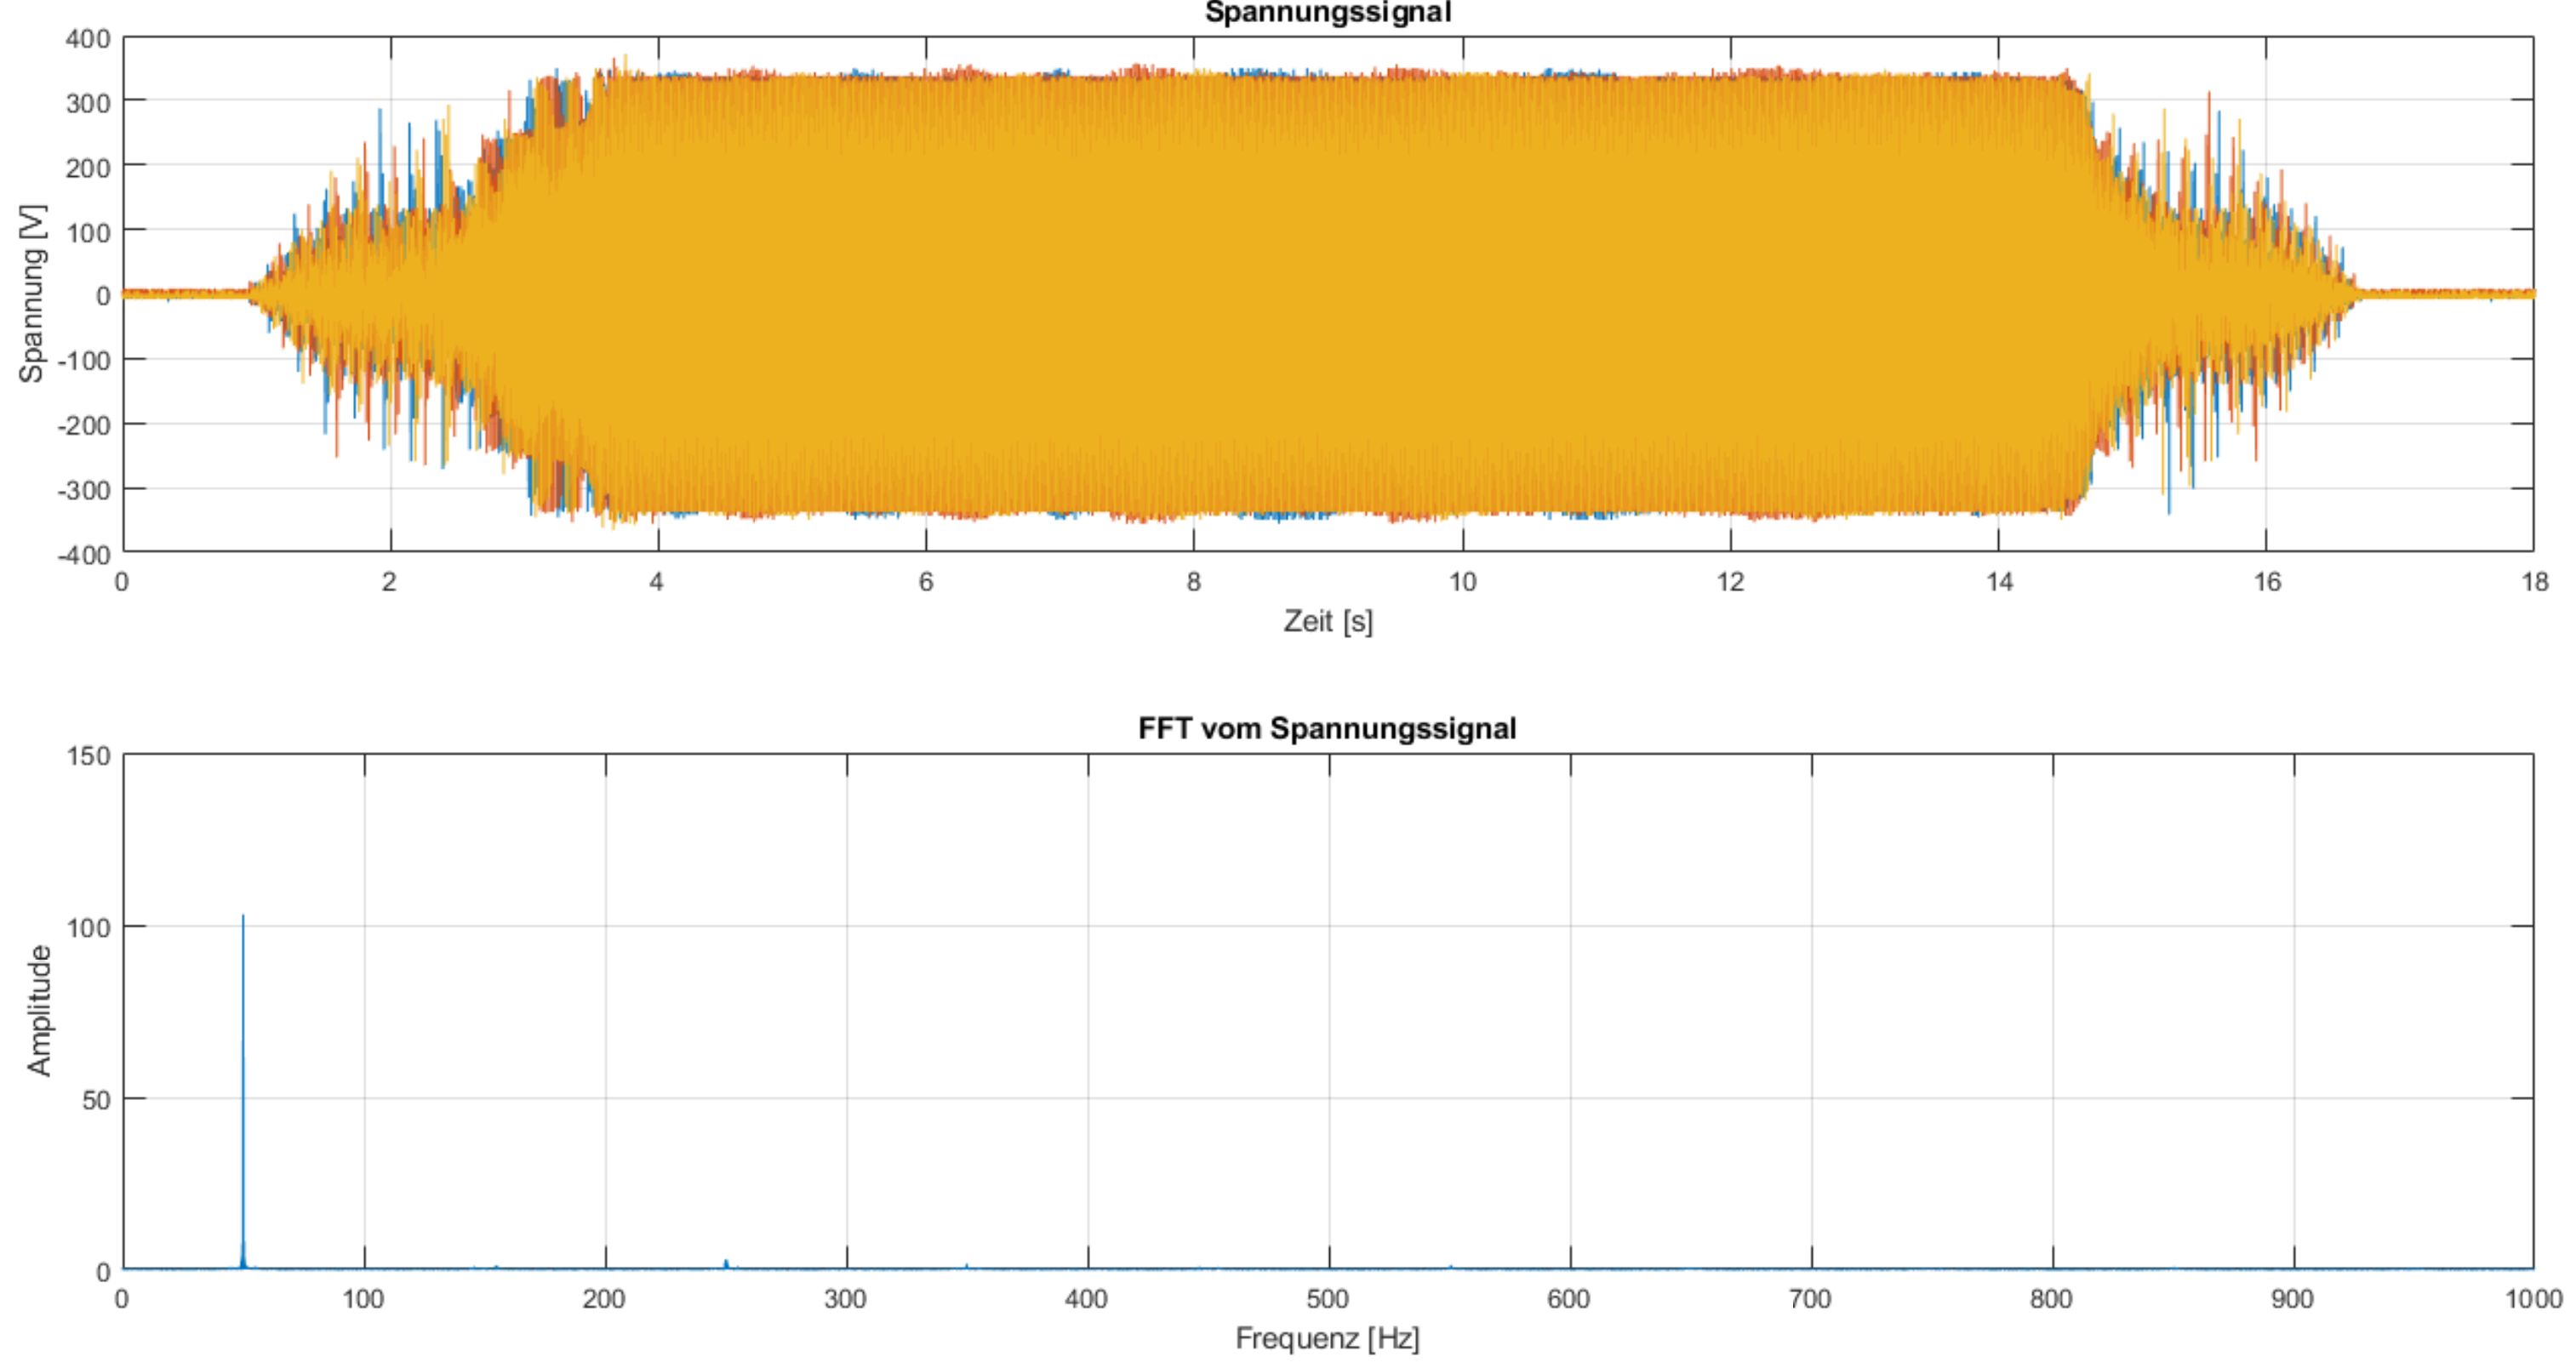
\includegraphics[width=\textwidth]{Messung_ASM_Sanft_langsam.png}	
	\caption{Messung mit Phasenanschnitt 90\textdegree}\label{fig:Mess_ASM_Sanft_langsam}
\end{figure}

\newpage
\subsubsection{Sanft-Anlasser Langsam}
\begin{figure}[ht!]
	\centering
	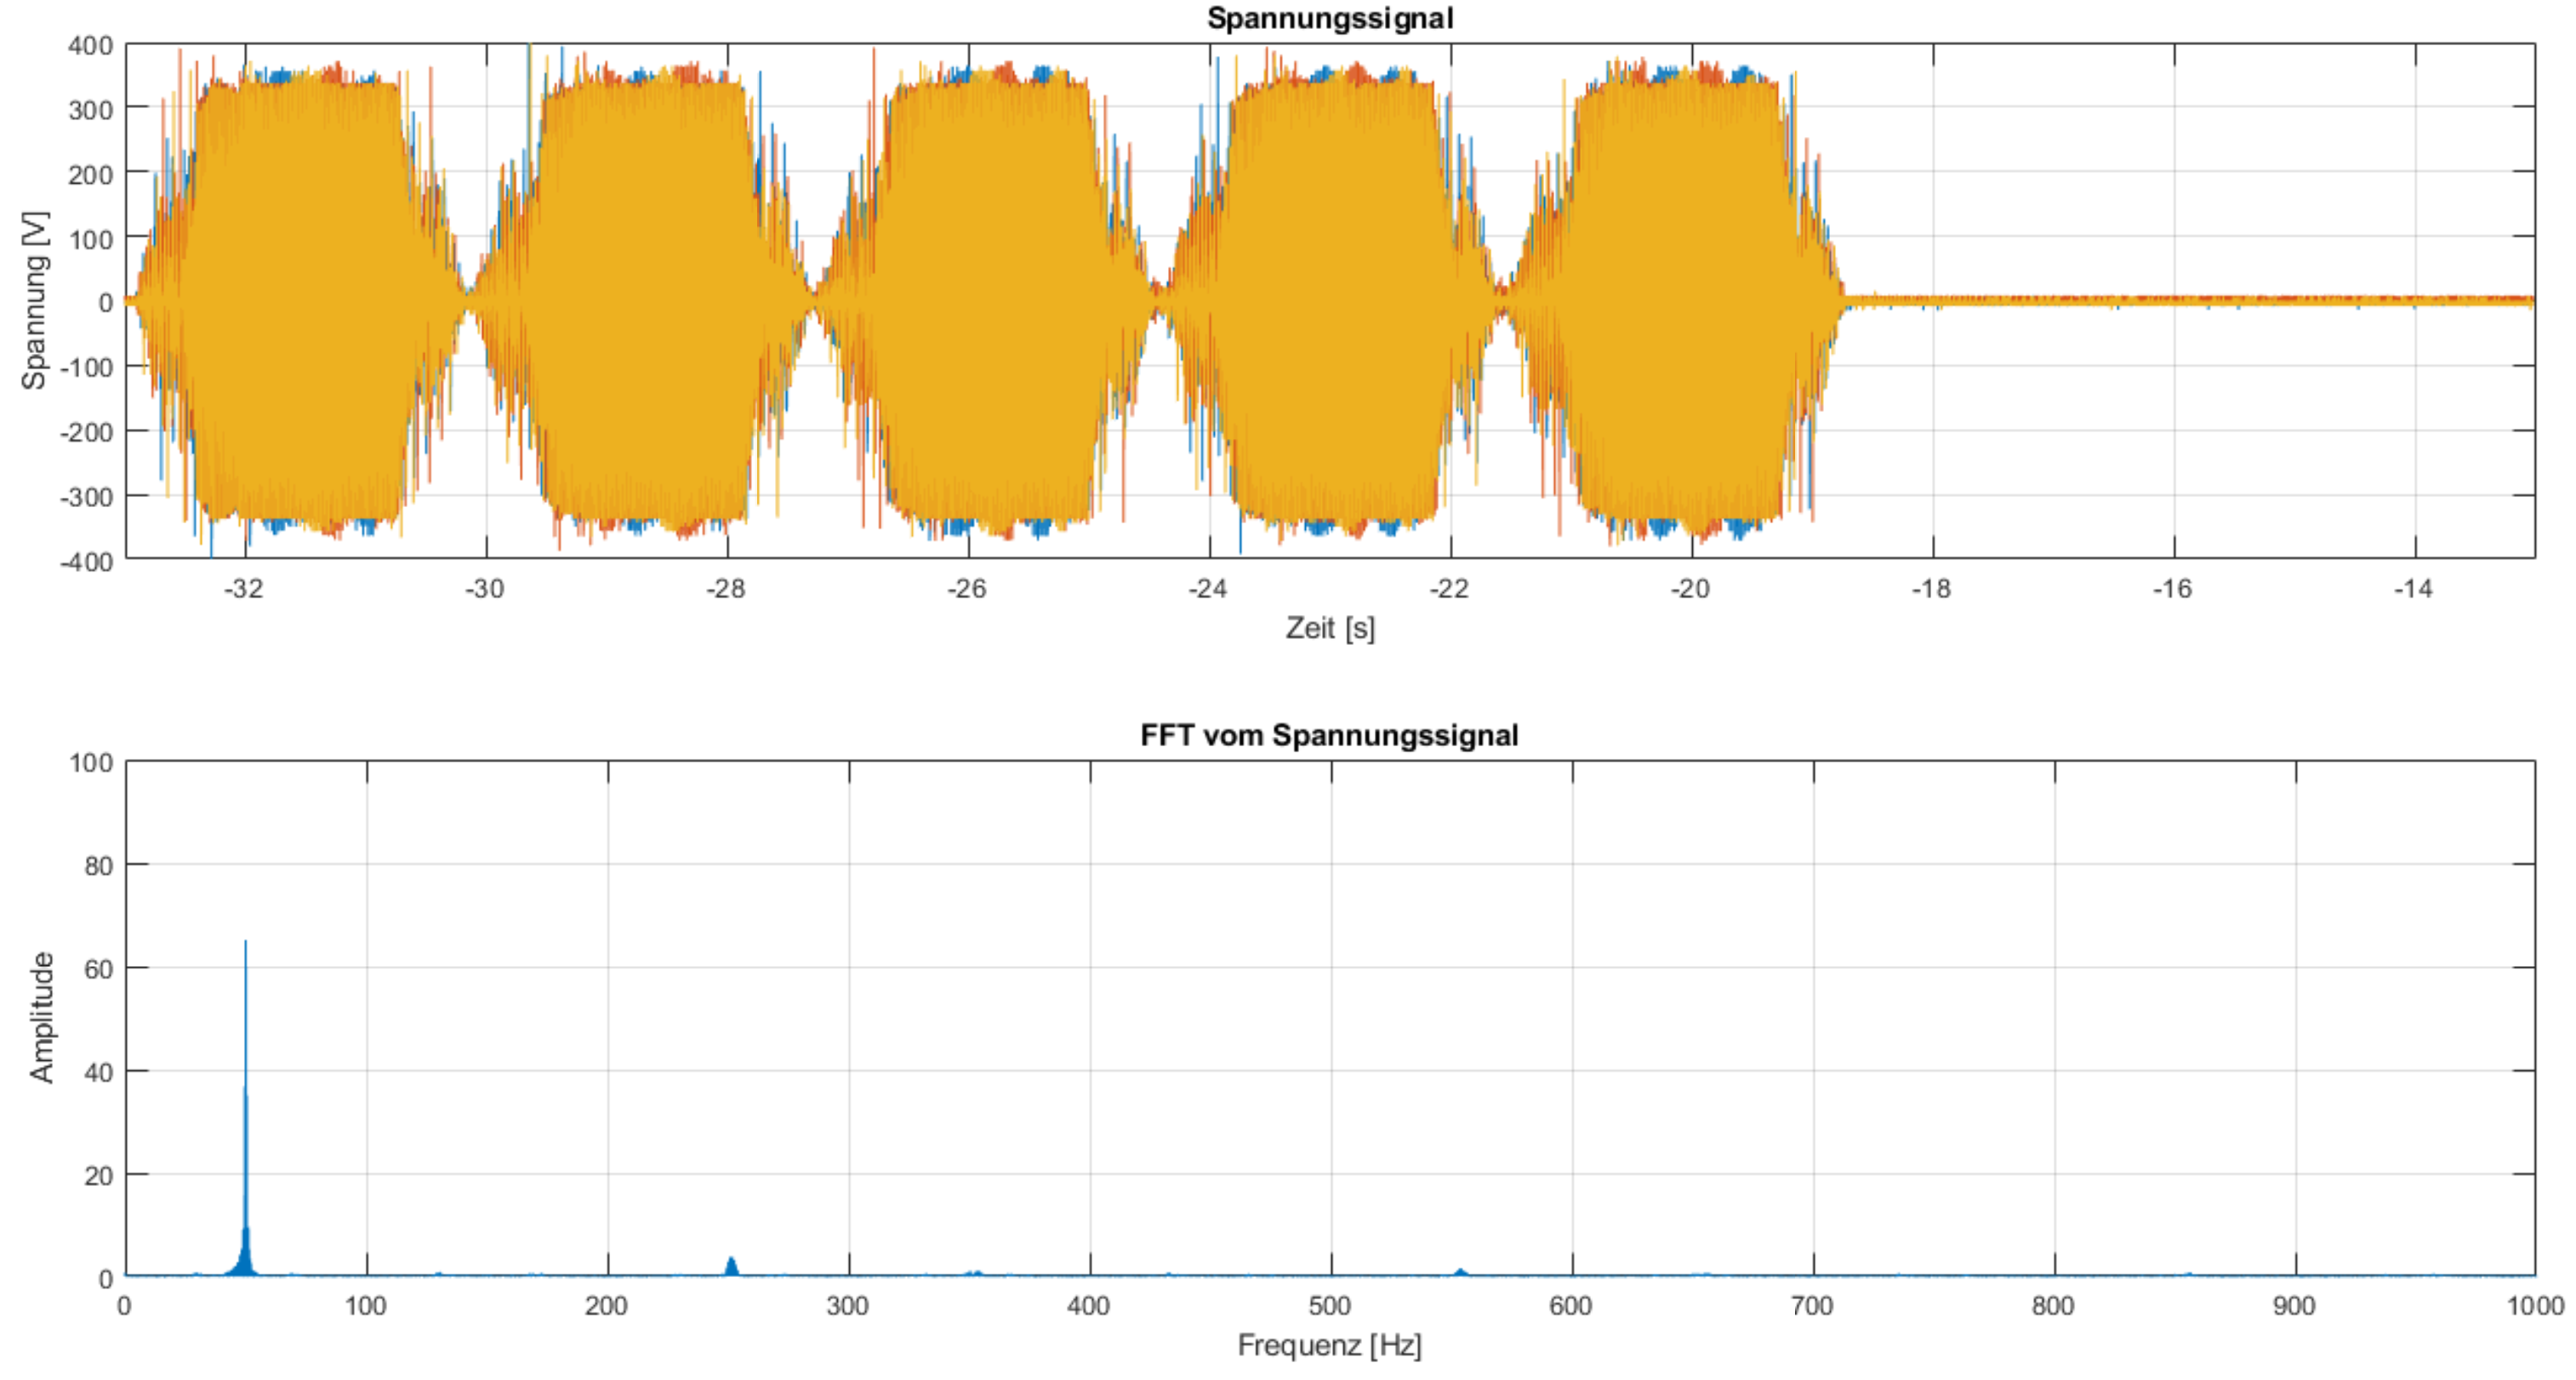
\includegraphics[width=\textwidth]{Messung_ASM_Sanft.png}	
	\caption{Messung mit Phasenanschnitt 90\textdegree}\label{fig:Mess_ASM_Sanft}
\end{figure}

%\subsubsection{Schwingungspaketsteuerung mit Last in Stern}
%Für die Messung mit der Schwingungspaketsteuerung wurde eine Einschaltzeit von 0.5 Sekunden und eine Ausschaltzeit von 0.2 Sekunden gewählt. Die Ausschaltzeit darf nicht kürzer sein, da die Spannungsverstärkerschaltung und den Thyristorsteller eine Zeitverzögerung darstellen und so die Spannung nicht sofort ein- oder ausgeschaltet wird. Wenn die Ausschaltzeit kürzer ist, geht die Spannung zwischen den Paketen nicht auf \SI{0}{V}. 
%\begin{figure}[ht!]
%	\centering
%	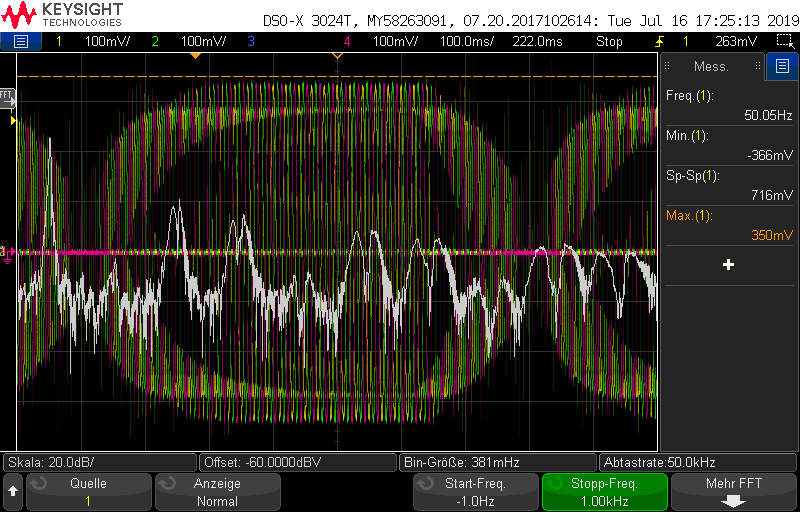
\includegraphics[width=0.7\textwidth]{Schwingungspaket_kurz.png}	
%	\caption{Das Spannungssignal aller Phasen bei Schwingungspaketsteuerung mit FFT}\label{fig:Mess_Schwing_kurz}
%\end{figure}
%
%Das FFT zeigt entgegen den Erwartungen aus der Theorie fast keine Subharmonische auf. Dafür sind Harmonische und Zwischehamrnische sehr ausgeprägt. Sehr gut zu sehen ist die Grundfrequenz von \SI{50}{Hz}, der erste Peak von der linken Seite. Dies ist darauf zurückzuführen, dass nicht direkt ein- und ausgeschaltet wird und so einem Sanft-Anlass ähnelt. Dies dominiert gegenüber dem harten Ein- und Ausschalten, welches die Subharmonische hervorrufen würde.
%\newpage
%\subsection{Phasenanschnittsteuerung mit 2 Thyristoren mit Last in Stern}
%Für die Sparansteuerung wurde ein Winkel von 90\textdegree \hspace{0.02cm} gewählt. 
%
%\begin{figure}[ht!]
%	\centering
%	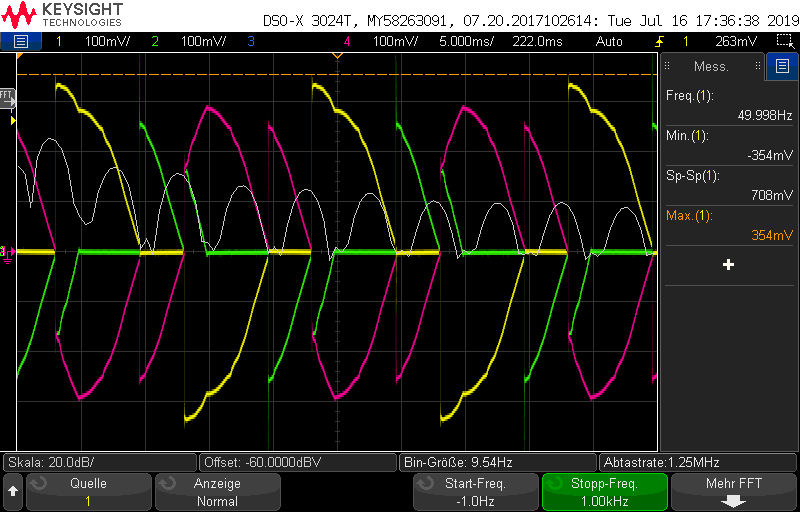
\includegraphics[width=0.7\textwidth]{2phas_90grad_kurz.png}	
%	\caption{Das Spannungssignal aller Phasen bei Schwingungspaketsteuerung mit FFT}\label{fig:Mess_2phas_kurz}
%\end{figure}
%
%
%\subsection{Phasenanschnittsteuerung mit 1 Thyristor mit Last in Stern}
%Für die Sparansteuerung wurde ein Winkel von 90\textdegree gewählt. 
%
%\begin{figure}[ht!]
%	\centering
%	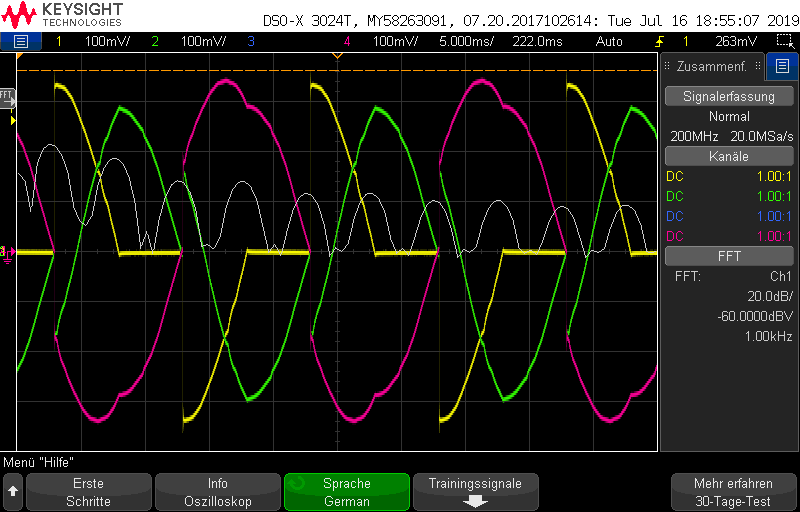
\includegraphics[width=0.7\textwidth]{1phas_90grad_kurz.png}	
%	\caption{Das Spannungssignal aller Phasen bei Schwingungspaketsteuerung mit FFT}\label{fig:Mess_1phas_kurz}
%\end{figure}




